\documentclass[10pt, openany, a5paper]{book}
% Set page size and margins
\usepackage[a5paper,top=1.5cm,bottom=2cm,left=2cm,right=2cm,marginparwidth=1.75cm]{geometry}
\usepackage[utf8]{inputenc}
\usepackage[T1]{fontenc}
\usepackage[portuguese]{babel}
\usepackage{amsmath, amsthm, amssymb}
\usepackage{fouriernc}
\usepackage{graphicx}

\graphicspath{{imagens/}} % Define o caminho padrão

\usepackage[dvipsnames]{xcolor}

\definecolor{mygreen}{rgb}{0,0.6,0}
\definecolor{mygray}{rgb}{0.5,0.5,0.5}
\definecolor{mymauve}{rgb}{0.58,0,0.82}

\usepackage{lipsum}
\usepackage{tocloft}

\usepackage{tikz}
\usepackage{pgfplots}
\usepackage{pgfplotstable}
\usetikzlibrary{shapes, arrows.meta, positioning, backgrounds} % Bibliotecas úteis

\pgfplotsset{compat=newest}
\usetikzlibrary{shapes.geometric, calc, arrows, shapes, trees}
\usetikzlibrary{arrows.meta}
\usepackage{tikz-3dplot} % Pacote para desenhos 3D
\usepackage[most]{tcolorbox}
\tcbuselibrary{skins,raster}
\usepackage{physics}
\usepackage{eso-pic}
\usepackage{ragged2e}
\usepackage{multicol}
\usepackage{lipsum}
\usepackage[shortlabels]{enumitem}
\usepackage{listings}

\lstset{
    language=tex,
    basicstyle=\ttfamily\small,
    keywordstyle=\color{blue},   
    commentstyle=\color{gray},  
    stringstyle=\color{red},   
    frame=single,               
    breaklines=true,            
    captionpos=b,               
}

\renewcommand{\lstlistingname}{Código}

\lstset{
    literate={á}{{\'a}}1 {é}{{\'e}}1 {í}{{\'i}}1 {ó}{{\'o}}1 {ú}{{\'u}}1
             {ã}{{\~a}}1 {õ}{{\~o}}1 {â}{{\^a}}1 {ê}{{\^e}}1 {ô}{{\^o}}1
             {À}{{\`A}}1 {à}{{\`a}}1 {ü}{{\"u}}1 {ç}{{\c{c}}}1 {Ç}{{\c{C}}}1
             {ö}{{\"o}}1
}

\usepackage{setspace}
\usepackage{tabularx}
\usepackage{multirow}
\usepackage{booktabs}
\usepackage{subcaption}
\usepackage{hyperref}

\definecolor{mylinkcolor}{HTML}{2D4802}  % Cor dos links internos
\definecolor{mycitecolor}{HTML}{8EB12D}  % Cor das citações
\definecolor{myurlcolor}{HTML}{638204}   % Cor dos links de URL

\hypersetup{
  linkcolor  = mylinkcolor, % Links internos (sumário, referências, etc.)
  citecolor  = mycitecolor, % Citações (quando usa \cite)
  urlcolor   = myurlcolor,  % Links externos
  colorlinks = true,        % Ativa cores nos links
}

\usepackage{cleveref}
\usepackage{filecontents}
\usepackage{fontawesome5}
\usetikzlibrary{shadows.blur} % Efeito de sombra
\usepackage{varwidth}

% --------------------------------------------------------
% ------------------------ CITAÇÕES ----------------------
% --------------------------------------------------------

% Comando para citação de abertura de capítulo com autor
\newcommand{\chapterquote}[2]{
  \begin{center}
    \small\textit{#1} \\ % A citação
    \vspace{0.5em} % Espaço entre a citação e o autor
    \small\textsc{--- #2} % O autor em small caps
  \end{center}
  \vspace{1em} % Espaçamento após a citação
}

% --------------------------------------------------------
% ------------------------ AMBIENTES ---------------------
% --------------------------------------------------------

% Contadores para cada tipo de ambiente
\newcounter{exercisecounter}
\newcounter{solutioncounter}

\newtcolorbox[auto counter]{exercisebox}[1][]{%
    beamer,
    enhanced, breakable, colback=white, % cor de fundo branca
    arc=5pt, outer arc=5pt,
    boxrule=0.5pt, colframe=black, % borda
    fontlower=\itshape,
    before=\vspace{2mm}, after=\vspace{2mm}, % Adiciona margem superior e inferior
    title={\small Questão~\thetcbcounter. #1}, % Adiciona o título com o contador e texto manual
    coltitle=white, % Define a cor do título para preto
}

\newtcolorbox[auto counter]{solutionbox}[1][]{%
	beamer,
    enhanced, breakable, colback=gray!10, colframe=gray!10,
    arc=10pt, outer arc=10pt,
    boxrule=0pt,
    before=\vspace{2mm}, after=\vspace{2mm},
    title={\small \textsc{Solução~\thetcbcounter}},
    coltitle=black, % Adiciona o título com o contador
    #1
}

\newtcolorbox{highlightbox}[1][]{%
	beamer,
    enhanced, breakable, colback=gray!10, colframe=gray!10, % cor de fundo atualizada para gray!10
    arc=0pt, outer arc=0pt,
    boxrule=0pt,
    before=\vspace{2mm}, after=\vspace{2mm},
    fonttitle=\bfseries\scshape, % Define o título em negrito e small caps
    coltitle=black, % Define a cor do título como preta
    #1}

% --------------------------------------------------------
% ------------------------ SUMÁRIO ---------------------
% --------------------------------------------------------

\addto\captionsportuguese{
  \renewcommand{\contentsname}{\hfill\bfseries\huge Sumário \hfill}   
}
\renewcommand{\cfttoctitlefont}{\hfill\bfseries\huge}
\renewcommand{\cftaftertoctitle}{\hfill\break\vspace{10pt}}

% Define o símbolo de quadrado preenchido
\newcommand{\filledsquare}{{\tikz{\node[fill=black,rectangle,minimum size=0.2cm] {};}}\hspace{0.5em}}

% Títulos de capítulos em negrito no sumário com o símbolo
\renewcommand{\cftchapfont}{\bfseries\large\filledsquare}

\begin{document}

% Primeira página com a imagem como background
\AddToShipoutPictureBG*{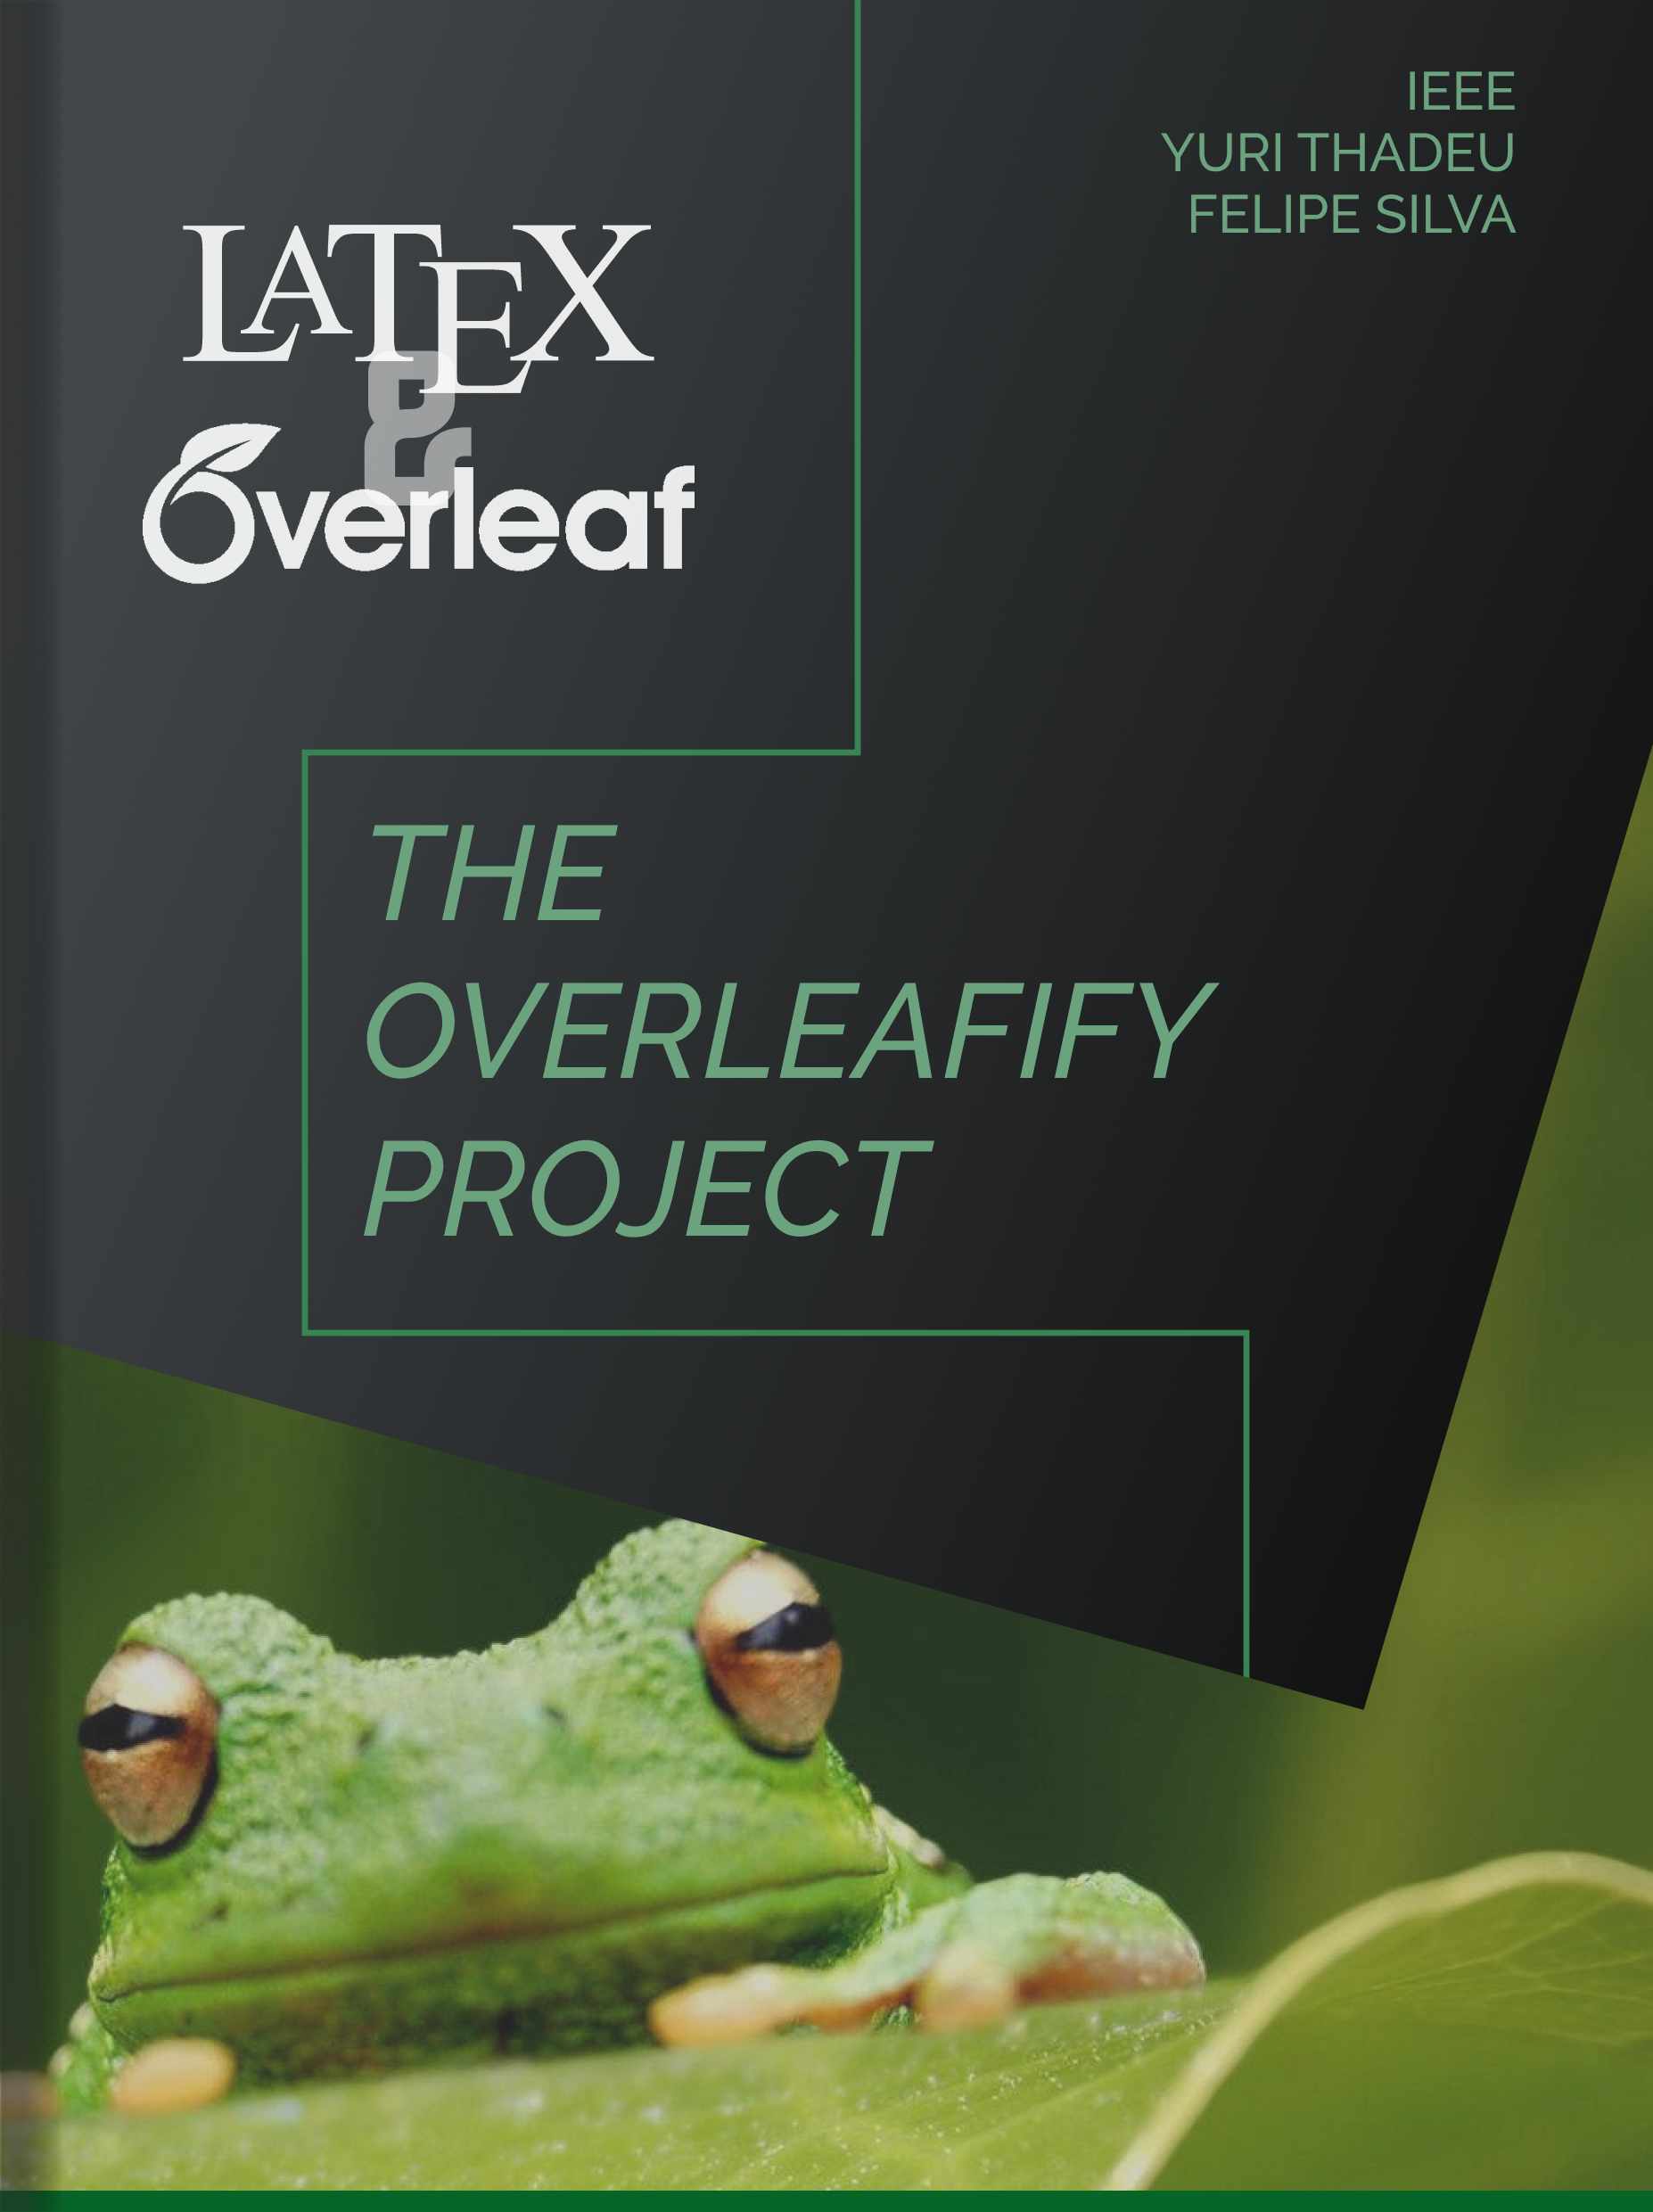
\includegraphics[width=\paperwidth,height=\paperheight]{capa.png}} % Substitua "capa.png" pelo nome real do arquivo da imagem
\begin{titlepage}
    \null % Adiciona um espaço vazio para que a imagem possa ser exibida corretamente
\end{titlepage}
\ClearShipoutPictureBG % Limpa o background da próxima página

\clearpage % Começa uma nova página para o conteúdo do livro

\thispagestyle{empty} % No page number on this page
\centering

\vspace{1cm} % Ajuste o espaço conforme necessário

{\Large\bfseries\textsc{\MakeUppercase{The Overleafify Project}}}\\[1cm]

{\large\textsc{Felipe Silva \& Yuri Thadeu}}\\
{IEEE}\\[20mm]  
\flushleft
\begin{minipage}{\textwidth}
\textsc{Resumo.} Este livro é um guia prático e acessível para iniciantes no uso do LaTeX e do Overleaf, ferramentas essenciais para a produção de documentos acadêmicos e técnicos de alta qualidade. Abordamos desde os conceitos básicos, como a estrutura de documentos e formatação de texto, até tópicos avançados, incluindo a criação de tabelas, inserção de imagens, expressões matemáticas, bibliografias e gráficos. Além disso, exploramos a criação de apresentações profissionais com o Beamer e a personalização de layouts para atender às necessidades específicas de cada projeto. Com exemplos práticos, exercícios e dicas úteis, este guia visa capacitar os novos ingressantes a dominar essas ferramentas de forma eficiente, tornando a documentação científica mais clara, organizada e esteticamente atraente.
\end{minipage}\\[1cm]   
\vfill
    \begin{center}
    	\textit{Copyright \copyright 2025, IEEE.}
    \end{center}
    \begin{center}
    	\textit{Este livro é distribuído sob uma licença aberta. A cópia, reprodução e compartilhamento são permitidos, desde que sejam mantidos os créditos aos autores.}
    \end{center}
\clearpage % Assegura que a próxima seção comece em uma nova página

\clearpage
\setcounter{page}{1} % Reseta o contador de páginas para o conteúdo principal

\thispagestyle{empty}
\tableofcontents

\pagestyle{empty} % Remove cabeçalho e rodapé

\chapter*{Prefácio}
\justify
\addcontentsline{toc}{chapter}{Prefácio}

O LaTeX é um sistema de preparação de documentos de alta qualidade, projetado para facilitar a criação de textos técnicos, científicos e acadêmicos. Diferentemente de editores de texto tradicionais, como o Microsoft Word, o LaTeX separa a formatação do conteúdo, permitindo que o autor se concentre na estrutura lógica do documento enquanto o sistema cuida da apresentação visual. Desenvolvido por Leslie Lamport na década de 1980, o LaTeX é construído sobre o TeX, um motor de tipografia criado por Donald Knuth, e tornou-se padrão em áreas como matemática, física, ciência da computação e engenharia, graças à sua precisão na renderização de fórmulas complexas e à capacidade de gerenciar referências cruzadas, bibliografias e índices de forma automatizada.

O Overleaf, por sua vez, é uma plataforma online que simplifica o uso do LaTeX, eliminando a necessidade de instalação local de compiladores e pacotes. Fundado em 2012, o Overleaf combina a potência do LaTeX com a praticidade de uma interface colaborativa em nuvem, permitindo que usuários escrevam, editem e compartilhem projetos em tempo real. Essa integração tornou-o popular em universidades e instituições de pesquisa, onde a colaboração em equipe e a padronização de documentos são essenciais.

Usar o Overleaf traz vantagens claras: além de acessível para iniciantes, ele oferece templates prontos, histórico de versões e integração com ferramentas como o Zotero e o GitHub. A plataforma também resolve um dos maiores desafios do LaTeX tradicional — a configuração inicial —, fornecendo ambientes pré-instalados e suporte a milhares de pacotes com um clique. Para estudantes e pesquisadores, isso significa menos tempo gasto em configurações técnicas e mais produtividade na escrita.

É importante reconhecer, porém, que o LaTeX pode parecer intimidador à primeira vista. Com sua sintaxe específica, inúmeros pacotes e curva de aprendizado, é fácil se perder em detalhes. Mas aqui está a chave: você não precisa dominar tudo de imediato. Comece com o básico — estrutura de documentos, formatação de texto, inserção de equações e referências — e avance gradualmente. À medida que ganhar confiança, explore templates criados pela comunidade para relatórios, artigos ou apresentações. Esses modelos não só aceleram seu trabalho como também servem de exemplo para aprender novos recursos.

Com o tempo, você perceberá que o LaTeX é uma ferramenta modular. Quando precisar de algo específico — como diagramas técnicos ou notação musical —, basta pesquisar o pacote adequado (ou perguntar a uma IA como o ChatGPT para sugerir soluções) e adaptá-lo ao seu projeto. Fóruns como o TeX Stack Exchange, comunidades no Reddit (r/LaTeX), grupos universitários de apoio ao LaTeX e até mesmo a seção de "Community" do Overleaf são recursos valiosos para tirar dúvidas, compartilhar projetos e se inspirar em soluções criativas. Aos poucos, você mesmo poderá criar seus próprios templates, combinando eficiência e estilo pessoal.

Por fim, é crucial entender a filosofia por trás do LaTeX: ele é um sistema WYSIWYM (What You See Is What You Mean), em contraste com editores WYSIWYG (What You See Is What You Get), como o Word. Enquanto no Word você ajusta visualmente cada elemento, no LaTeX você define a intenção do conteúdo (por exemplo, "isto é um título", "isto é uma equação"), e o sistema cuida da formatação. Isso pode exigir um investimento inicial de tempo, mas evita retrabalhos infinitos com ajustes estéticos. A dica é: não se perca em personalizações desnecessárias. Siga boas práticas, use pacotes consagrados e priorize a clareza. O LaTeX foi feito para ser prático — e, com as ferramentas certas, ele será.

\clearpage
\pagestyle{plain} % Restaura o estilo de página padrão para o restante do documento

\chapter{Tipos de documentos e estruturas}

\chapterquote{``Citação.''}{Autor}

% --------

\section{Classes de documentos no LaTeX}

O LaTeX oferece diferentes classes de documentos para atender a diversos propósitos. As principais são:
\begin{enumerate}
    \item \verb|article|: Ideal para artigos científicos, relatórios curtos e documentos simples.
    \begin{lstlisting}[language=tex]
    \documentclass[a4paper, 12pt]{article} % Tamanho A4, fonte 12pt
    \end{lstlisting}
    \item \verb|report|: Usado para relatórios técnicos, monografias ou documentos com capítulos.
    \begin{lstlisting}[language=tex]
    \documentclass[a4paper, 12pt]{report}
    \end{lstlisting}
    \item \verb|book|: Projetado para livros, teses e dissertações, com suporte a capítulos, partes e elementos pré-textuais.
    \begin{lstlisting}[language=tex]
    \documentclass[a4paper, 12pt]{book}
    \end{lstlisting}
    \item \verb|beamer|: Para criar apresentações de slides.
    \begin{lstlisting}[language=tex]
    \documentclass{beamer}
    \end{lstlisting}
\end{enumerate}

\section{Estrutura básica de um documento}
Todo documento em LaTeX possui três partes principais:
\begin{enumerate}
    \item \textbf{Pré-âmbulo}: Define a classe, pacotes e configurações globais.
    \item \textbf{Corpo}: Contém o conteúdo visível do documento.
    \item \textbf{Pós-âmbulo} (opcional): Inclui apêndices, glossários ou índices.
\end{enumerate}

\begin{lstlisting}[language=tex, caption=Exemplo de estrutura mínima]
    \documentclass{article} % Pré-âmbulo
    \begin{document}         % Início do corpo
        Olá, mundo!          % Conteúdo
    \end{document}           % Fim do corpo
\end{lstlisting}

\section{Elementos específicos por classe}

\subsection{Artigo (\texttt{article})}
\begin{itemize}
    \item Capa simples, resumo (\textit{abstract}), seções (sem capítulos)
    \begin{lstlisting}[language=tex, caption=Exemplo de artigo]
    \documentclass{article}
    \title{Meu Artigo}
    \author{Fulano}
    \date{\today}
    \begin{document}
        \maketitle
        \begin{abstract}
            Resumo do artigo...
        \end{abstract}
        \section{Introdução}
            Texto da introdução...
    \end{document}
    \end{lstlisting}
\end{itemize}

\subsection{Livro (\texttt{book})}

\begin{itemize}
    \item Divisão clara entre elementos pré-textuais (\verb|\frontmatter|) e o corpo (\verb|\mainmatter|).
    \begin{lstlisting}[language=tex, caption=Exemplo de livro]
    \documentclass{book}
    \title{Meu Livro}
    \author{Fulano}
    \begin{document}
        \frontmatter       % Pré-texto (numeração romana)
            \maketitle
            \tableofcontents
        \mainmatter        % Corpo (numeração arábica)
            \chapter{Introdução}
                Texto...
    \end{document}
    \end{lstlisting}
\end{itemize}

\section{Geometria da página}

Use o pacote \verb|geometry| para ajustar margens:

\begin{lstlisting}[language=tex, caption=Ajuste das margens com o pacote \texttt{geometry}]
    \usepackage[top=3cm, left=3cm, right=2cm, bottom=2cm]{geometry}
\end{lstlisting}

\section{Dicas práticas}

\begin{itemize}
    \item Pacotes essenciais:
    \begin{lstlisting}[language=tex, caption=Pacotes mais fundamentais]
    \usepackage[brazilian]{babel}     % Traduz termos para português
    \usepackage[utf8]{inputenc}      % Suporte a acentuação
    \usepackage{amsmath}             % Fórmulas matemáticas
    \end{lstlisting}
    \item Erros comuns:
    \begin{itemize}
        \item Não fechar ambientes (\verb|\begin{document} ...\end{document}|).
        \item Usar \verb|\chapter| em classes que não suportam (como \verb|article|).
    \end{itemize}
\end{itemize}

\chapter{Texto e formatação}

\chapterquote{``Citação.''}{Autor}

% --------

\section{Formatação básica}

\begin{itemize}
    \item \textbf{Negrito}: \verb|\textbf{Texto em negrito}|
    \item \textit{Itálico}: \verb|\textit{Texto em itálico}|
    \item \underline{Sublinhado}: \verb|\underline{Texto sublinhado}|
\end{itemize}

\begin{lstlisting}[language=tex, caption=Formatação básica de texto]
    \textbf{Importante}: \textit{Não esqueça} de \underline{revisar} o código.
\end{lstlisting}

O código acima gera como saída:\\

\textbf{Importante}: \textit{Não esqueça} de \underline{revisar} o código.

\section{Tamanhos da fonte}

Tamanhos pré-definidos (do menor ao maior):
{\tiny Texto pequeno}  
{\scriptsize Um pouco maior}  
{\footnotesize Notas de rodapé}  
{\small Pequeno}  
{\normalsize Normal}  
{\large Grande}  
{\Large Maior}  
{\LARGE Muito grande}  
{\huge Enorme}  
{\Huge Gigante}

\begin{lstlisting}[language=tex, caption=Tamanhos de fontes pré-definidos]
    {\tiny Texto pequeno}  
    {\scriptsize Um pouco maior}  
    {\footnotesize Notas de rodapé}  
    {\small Pequeno}  
    {\normalsize Normal}  
    {\large Grande}  
    {\Large Maior}  
    {\LARGE Muito grande}  
    {\huge Enorme}  
    {\Huge Gigante}  
\end{lstlisting}

Dica: Use \verb|\normalsize| para voltar ao tamanho padrão após alterações.

\section{Cores no texto}

Use o pacote \verb|xcolor|:

\begin{lstlisting}[language=tex, caption=Uso do pacote \texttt{xcolor} para customização de cores no texto]
    \usepackage{xcolor}  
    \textcolor{red}{Texto vermelho}  
    \textcolor{blue}{Texto azul}  
    \textcolor[HTML]{00FF00}{Verde em hexadecimal}  
\end{lstlisting}

\textcolor{red}{Texto vermelho}  
\textcolor{blue}{Texto azul}  
\textcolor[HTML]{00FF00}{Verde em hexadecimal}  

\section{Listas}

\subsection{Listas enumeradas - ambiente \texttt{enumerate}}

\begin{lstlisting}[language=tex, caption=Listas enumeradas]
    \begin{enumerate}
        \item Primeiro item
        \item Segundo item
    \end{enumerate} 
\end{lstlisting}

\begin{enumerate}
    \item Primeiro item
    \item Segundo item
\end{enumerate}

\subsection{Listas não enumeradas - ambiente \texttt{itemize}}

\begin{lstlisting}[language=tex, caption=Listas não enumeradas]
    \begin{itemize}
        \item Item com marcador padrão
        \item Outro item
    \end{itemize}
\end{lstlisting}

\begin{itemize}
    \item Item com marcador padrão
    \item Outro item
\end{itemize}

\subsection{Listas descritivas - ambiente \texttt{description}}

\begin{lstlisting}[language=tex, caption=Listas descritivas]
    \begin{description}
        \item[LaTeX] Sistema de preparação de documentos.
        \item[Overleaf] Plataforma online para LaTeX.
    \end{description}
\end{lstlisting}

\begin{description}
    \item[LaTeX] Sistema de preparação de documentos.
    \item[Overleaf] Plataforma online para LaTeX.
\end{description}

Dica: Use o pacote \verb|enumitem| para personalizar marcadores e espaçamento.

\section{Espaçamento e parágrafos}
\begin{itemize}
    \item Quebra de linha: \verb|\\| ou \verb|\newline|
    \item Novo parágrafo: Deixe uma linha vazia no código ou use \verb|\par|.
    \item Espaçamento vertical: \verb|\vspace{1cm}|
    \item Espaçamento horizontal: \verb|\hspace{2em}|
\end{itemize}

\begin{lstlisting}[language=tex, caption=Exemplo de espaçamento e parágrafos]
    Primeira linha.\\ Segunda linha.  
    \par Terceira linha (novo parágrafo).
\end{lstlisting}

Primeira linha.\\ Segunda linha.  
\par Terceira linha (novo parágrafo).

% \section{Espaçamento entre linhas}

% Use o pacote \verb|setspace|:

\section{Dicas práticas}

\begin{itemize}
    \item Pacotes úteis:
    \begin{lstlisting}[language=tex, caption=Outros pacotes úteis para texto e formatação]
    \usepackage{lipsum}   % Gerar texto aleatório para testes
    \usepackage{hyperref} % Links clicáveis
    \end{lstlisting}
    \item Erros comuns:
    \begin{itemize}
        \item Esquecer de fechar chaves \verb|{}| após comandos de formatação.
        \item Usar \verb|\\| excessivamente (pode causar layout quebrado).
    \end{itemize}
\end{itemize}


\chapter{Criação de tabelas}

\chapterquote{``Citação.''}{Autor}

% --------

\section{Tabelas básicas com \texttt{tabular}}

O ambiente \verb|tabular| é a base para criar tabelas em LaTeX.

\begin{lstlisting}[language=tex, caption=Sintaxe básica para criação de tabelas]
    \begin{tabular}{colunas}
        Conteúdo das células & separado por & \\
        Linhas separadas por \\ 
    \end{tabular}
\end{lstlisting}

\begin{lstlisting}[language=tex, caption=Exemplo básico de tabela]
    \begin{center}
        \begin{tabular}{|c|c|c|}  % Colunas centralizadas (c) com bordas (|)
            \hline
            Nome & Idade & Cidade \\ 
            \hline
            João & 25 & São Paulo \\ 
            Maria & 30 & Rio de Janeiro \\ 
            \hline
        \end{tabular}
    \end{center}
\end{lstlisting}

\begin{center}
    \begin{tabular}{|c|c|c|}  % Colunas centralizadas (c) com bordas (|)
        \hline
        Nome & Idade & Cidade \\ 
        \hline
        João & 25 & São Paulo \\ 
        Maria & 30 & Rio de Janeiro \\ 
        \hline
    \end{tabular}
\end{center}

\section{Tipos de colunas}

\begin{itemize}
    \item \verb|c|: Centralizada.
    \item \verb|l|: Alinhada à esquerda.
    \item \verb|r|: Alinhada à direita;
    \item \verb|||: Adiciona bordas verticais
    \item \verb|p{largura}|: Coluna com largura fixa
\end{itemize}

\begin{lstlisting}[language=tex, caption=Exemplo com alinhamento]
    \begin{tabular}{l r p{4cm}}
        Nome (esquerda) & Preço (direita) & Descrição (largura fixa) \\ 
        \hline
        Livro & R\$ 50,00 & Um livro sobre LaTeX \\ 
        Caneta & R\$ 2,50 & Caneta azul \\ 
    \end{tabular}
\end{lstlisting}

\begin{tabular}{l r p{4cm}}
    Nome (esquerda) & Preço (direita) & Descrição (largura fixa) \\ 
    \hline
    Livro & R\$ 50,00 & Um livro sobre LaTeX \\ 
    Caneta & R\$ 2,50 & Caneta azul \\ 
\end{tabular}

\section{Pacote \texttt{tabularx} para largura ajustável}

Permite criar tabelas que se ajustam à largura do texto.

\begin{lstlisting}[language=tex, caption=Uso do pacote \texttt{tabularx}]
\begin{tabularx}{\textwidth}{|X|X|X|} % Colunas X dividem o espaço igualmente
    \hline
    Cabeçalho 1 & Cabeçalho 2 & Cabeçalho 3 \\ 
    \hline
    Texto longo que se ajusta automaticamente & Dado 2 & Dado 3 \\ 
    \hline
\end{tabularx}
\end{lstlisting}

\section{Linhas horizontais e verticais}

\begin{itemize}
    \item \verb|\hline|: Linha horizontal.
    \item \verb|cline{i-j}|: Linha horizontal parcial.
    \item \verb|||: Bordas verticais (ex: \texttt{|c|c|c|}).
\end{itemize}

\begin{lstlisting}[language=tex, caption=Exemplo de criação de tabela]
    \begin{center}
        \begin{tabular}{|l|c|r|}
            \hline
            \multicolumn{3}{|c|}{Título da Tabela} \\ 
            \hline
            Item & Quantidade & Preço \\ 
            \cline{1-2} % Linha parcial
            Livro & 2 & R\$ 100,00 \\ 
            \hline
        \end{tabular}
    \end{center}
\end{lstlisting}

\begin{center}
    \begin{tabular}{|l|c|r|}
        \hline
        \multicolumn{3}{|c|}{Título da Tabela} \\ 
        \hline
        Item & Quantidade & Preço \\ 
        \cline{1-2} % Linha parcial
        Livro & 2 & R\$ 100,00 \\ 
        \hline
    \end{tabular}
\end{center}

\section{Mesclando células}

\begin{itemize}
    \item \verb|\multicolumn{n}{alinhamento}{texto}|: Mescla colunas.
    \item \verb|\multirow{n}{largura}{texto}|: Mescla linhas (requer o pacote \verb|multirow|).
\end{itemize}

\begin{lstlisting}[language=tex, caption=Exemplo de mesclagem]
\begin{center}
    \begin{tabular}{|c|c|c|}
        \hline
        \multirow{2}{*}{Categoria} & \multicolumn{2}{c|}{Dados} \\ 
        \cline{2-3}
        & Produto & Preço \\ 
        \hline
        Livros & LaTeX Guide & R\$ 80,00 \\ 
        \hline
    \end{tabular}
\end{center}
\end{lstlisting}

\begin{center}
    \begin{tabular}{|c|c|c|}
        \hline
        \multirow{2}{*}{Categoria} & \multicolumn{2}{c|}{Dados} \\ 
        \cline{2-3}
        & Produto & Preço \\ 
        \hline
        Livros & LaTeX Guide & R\$ 80,00 \\ 
        \hline
    \end{tabular}
\end{center}

\section{Tabelas profissionais com \texttt{booktabs}}

O pacote \verb|booktabs| remove bordas excessivas e melhora a estética:

\begin{lstlisting}[language=tex, caption=Exemplo de mesclagem]
\begin{center}
    \begin{tabular}{lcc}
        \toprule
        Nome & Nota 1 & Nota 2 \\ 
        \midrule
        João & 8,5 & 9,0 \\ 
        Maria & 7,0 & 8,5 \\ 
        \bottomrule
    \end{tabular}
\end{center}
\end{lstlisting}

\begin{center}
    \begin{tabular}{lcc}
        \toprule
        Nome & Nota 1 & Nota 2 \\ 
        \midrule
        João & 8,5 & 9,0 \\ 
        Maria & 7,0 & 8,5 \\ 
        \bottomrule
    \end{tabular}
\end{center}

Dica: Evite usar \verb|\hline| com \verb|booktabs| para manter o estilo limpo.

\section{Dicas práticas}

\begin{itemize}
    \item Pacotes úteis:
    \begin{lstlisting}[language=tex, caption=Pacotes úteis e interessantes para usar com tabelas]
    \usepackage{array}       % Mais controle sobre colunas
    \usepackage{graphicx}    % Inserir imagens em células
    \end{lstlisting}
    \item Erros comuns:
    \begin{itemize}
        \item Esquecer de adicionar \& entre células.
        \item Usar \verb|\\| no final da última linha (desnecessário).
    \end{itemize}
\end{itemize}
    

\chapter{Manipulação de Imagens em LaTeX}

\chapterquote{``Citação.''}{Autor}

% --------

\section{Introdução ao pacote \texttt{graphicx}}

O pacote \verb|graphicx| é essencial para inserir imagens. Carregue-o no pré-âmbulo:

\begin{lstlisting}[language=tex, caption=Carregue o pacote \texttt{graphicx}]
    \usepackage{graphicx} % Sempre adicione isso!
\end{lstlisting}

Formato de imagens suportados:
\begin{itemize}
    \item \textbf{Overleaf}: \verb|PNG|, \verb|JPG|, \verb|PDF| (evite \verb|SVG|, a menos que convertido.
    \item \textbf{LaTeX offline}: \verb|PDF|, \verb|EPS|, \verb|PNG|, \verb|JPG|
\end{itemize}

\section{Inserindo imagens básicas}

Use \verb|\includegraphics| para adicionar uma imagem:

\begin{lstlisting}[language=tex, caption=Inserindo uma imagem]
    \includegraphics[width=0.5\textwidth]{caminho/para/imagem.png}  
\end{lstlisting}

\section{Redimensionamento e escala}

\begin{itemize}
    \item Largura fixa: \verb|width=8cm|.
    \item Altura fixa: \verb|height=4cm|.
    \item Escala proporcional: \verb|scale=0.7|.
    \item Rotação: \verb|angle=45|
\end{itemize}

\begin{lstlisting}[language=tex, caption=Exemplo de customização do tamanho e ângulo de imagem]
    \includegraphics[width=5cm, angle=30]{imagem.jpg}  
\end{lstlisting}

\newpage

\section{Posicionamento com o ambiente \texttt{figure}}

O ambiente \verb|figure| permite controle profissional sobre posição, legendas e referências:

\begin{lstlisting}[language=tex, caption=Exemplo de customização do tamanho e ângulo de imagem]
    \begin{figure}[h!] % Opções: h (aqui), t (topo), b (base), p (página separada)
        \centering
        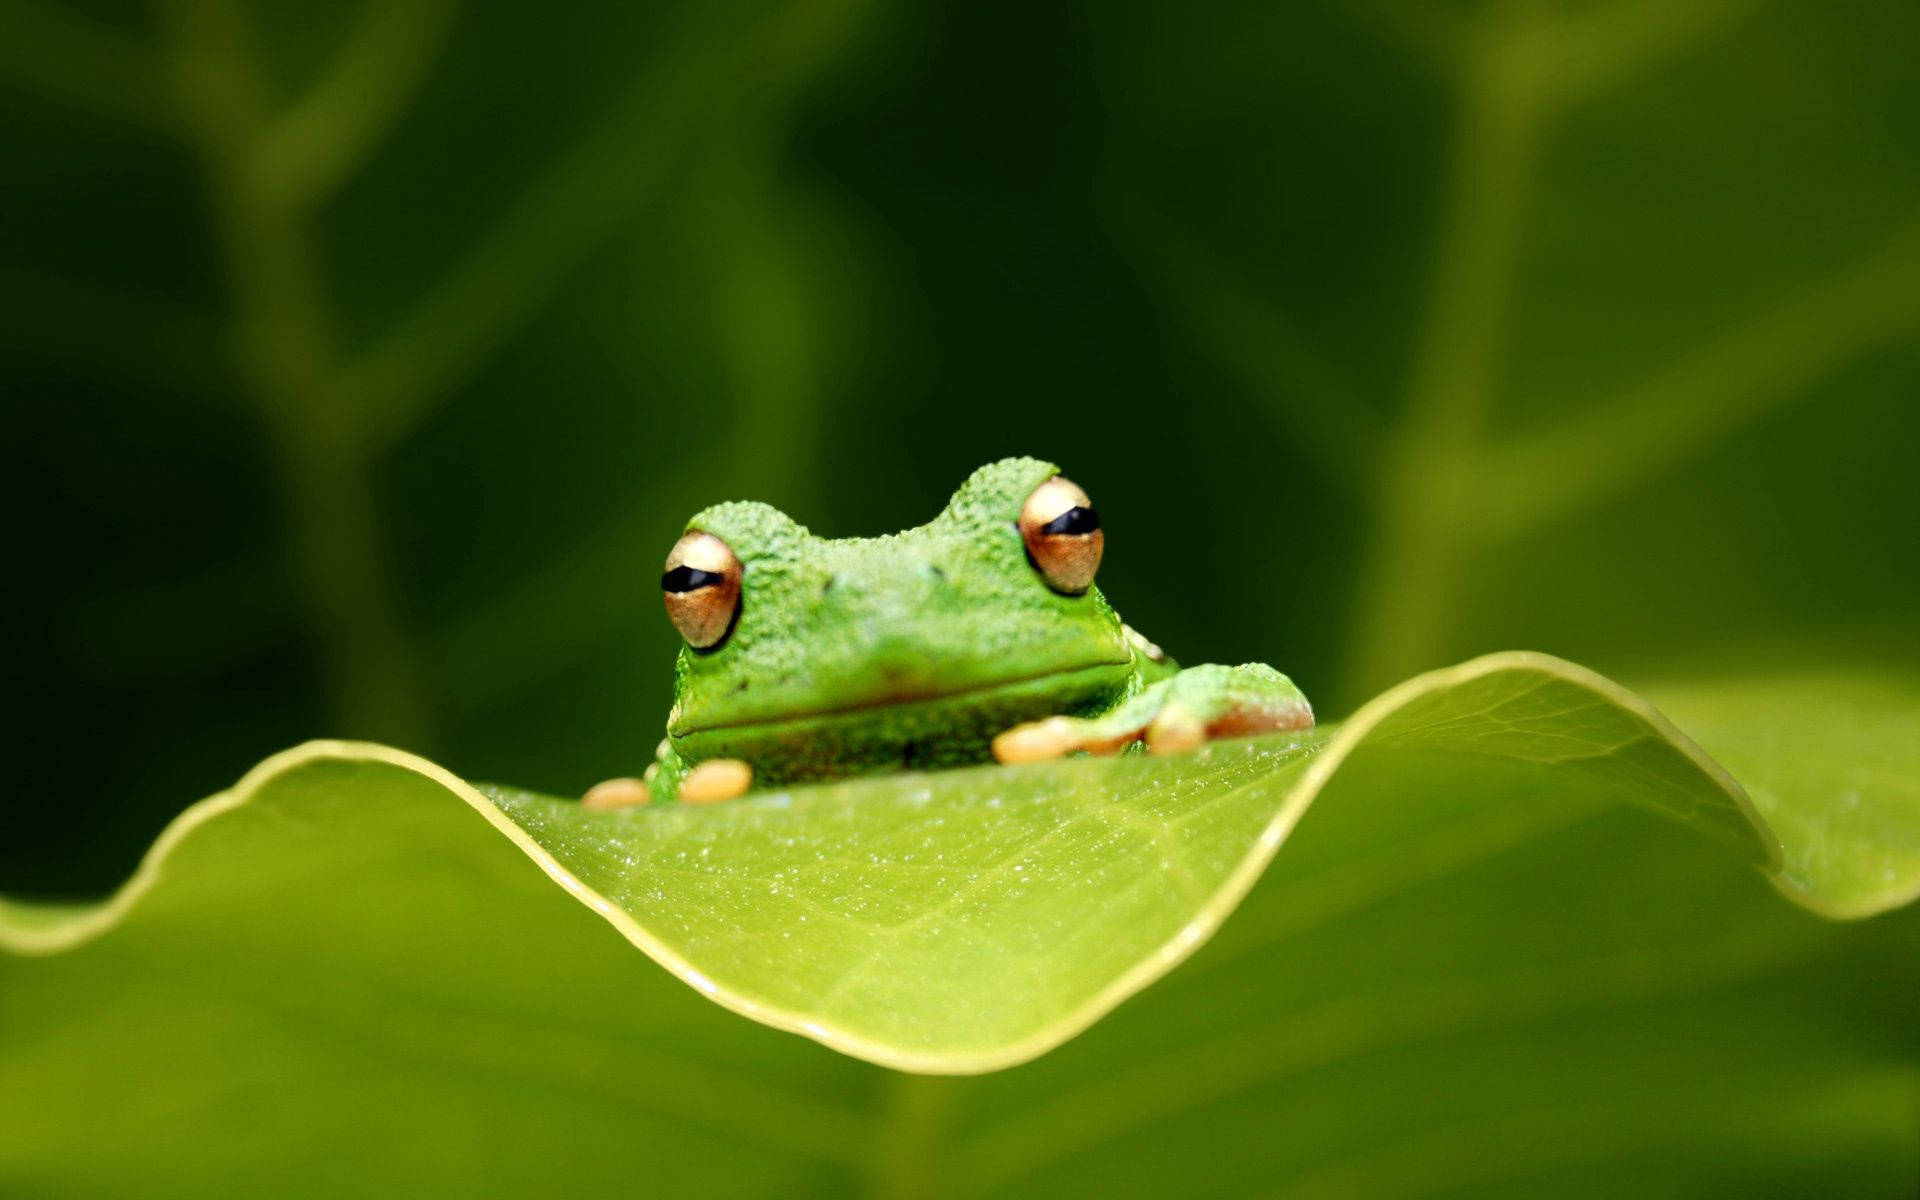
\includegraphics[width=0.4\textwidth]{imagens/sapo.jpg}
        \caption{Imagem da capa do livro} % Legenda
        \label{fig:sapodacapa} % Rótulo para referência
    \end{figure}
\end{lstlisting}

\begin{figure}[h!] % Opções: h (aqui), t (topo), b (base), p (página separada)
    \centering
    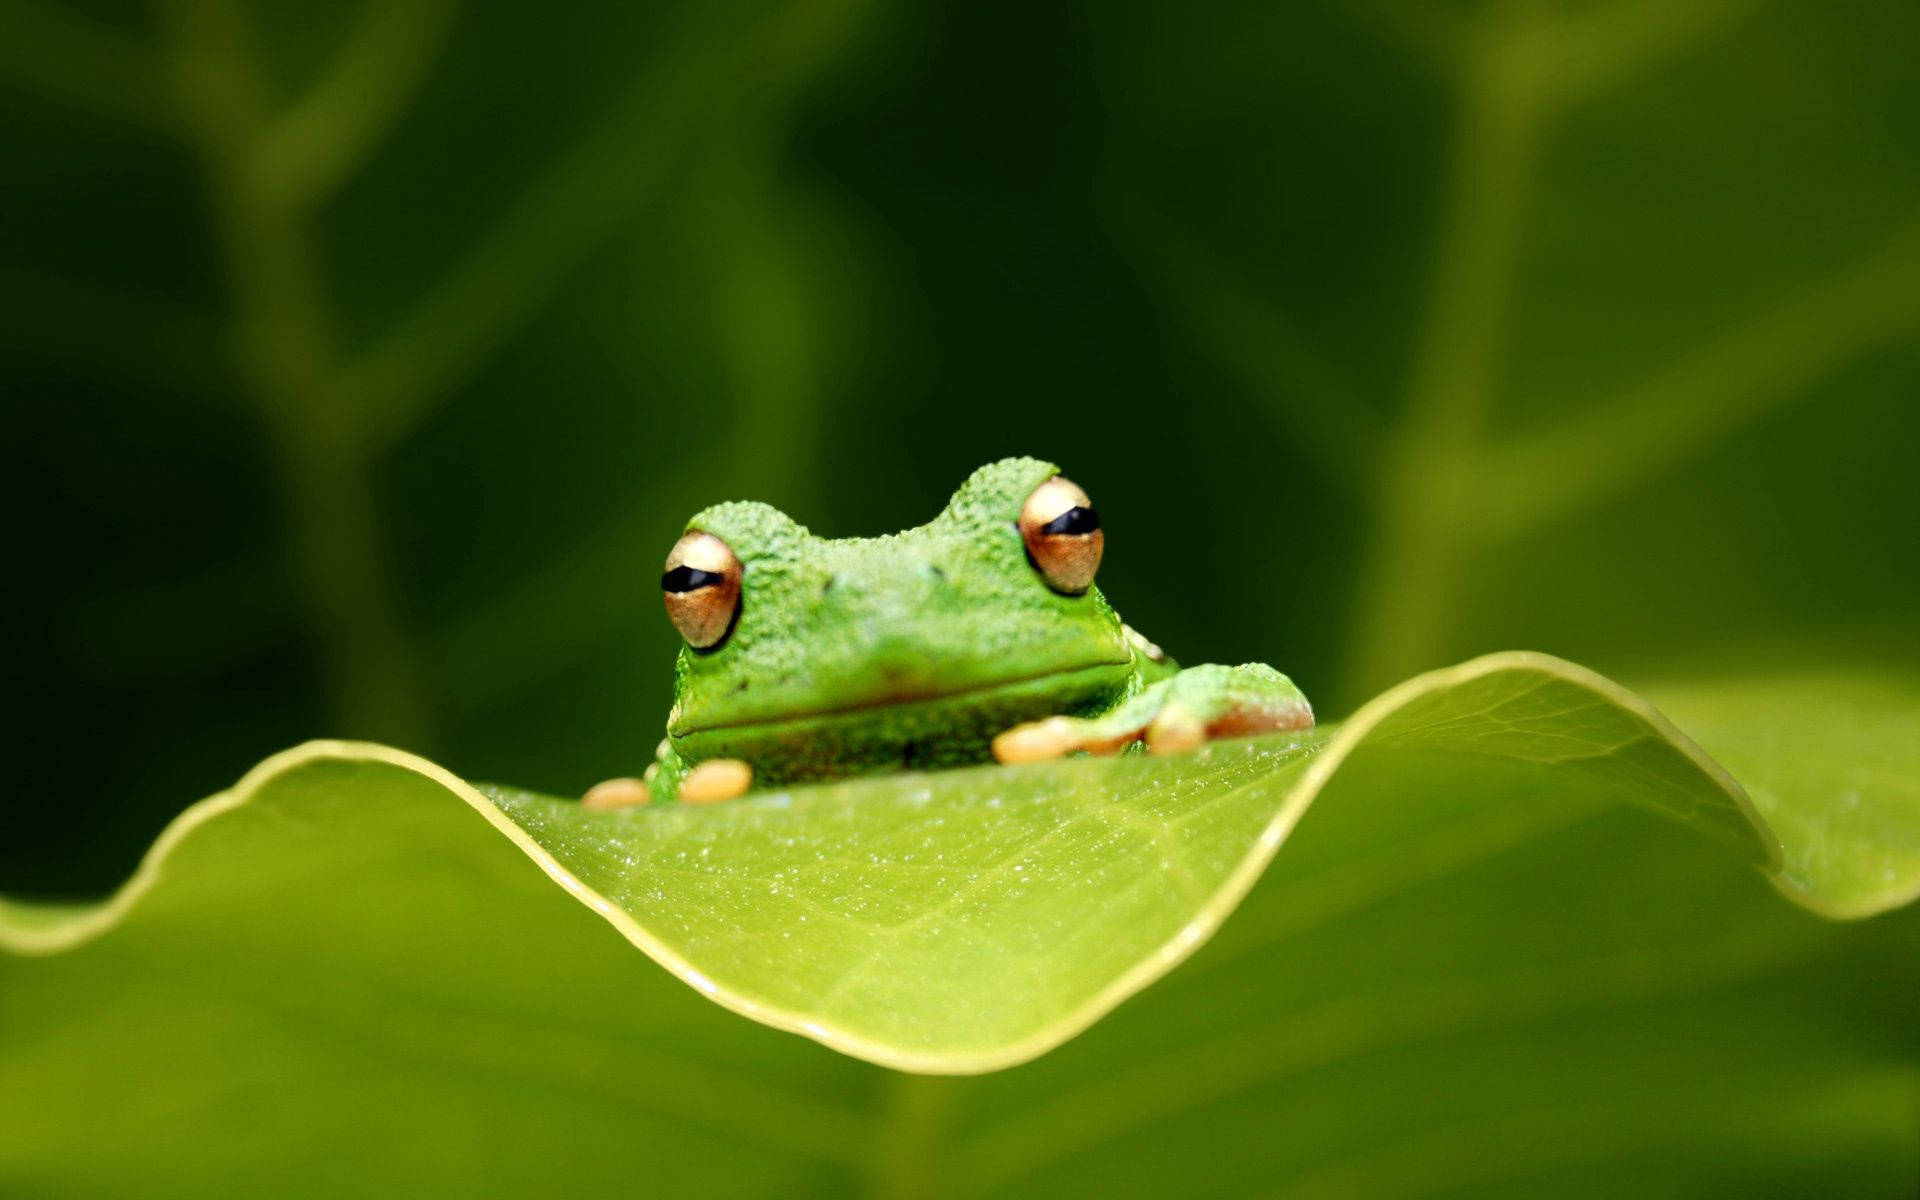
\includegraphics[width=0.7\textwidth]{imagens/sapo.jpg}
    \caption{Imagem da capa do livro} % Legenda
    \label{fig:sapodacapa} % Rótulo para referência
\end{figure}

\section{Múltiplas imagens em uma figura}

Use o pacote \verb|subcaption| para criar subfiguras:

\begin{lstlisting}[language=tex, caption=Exemplo de customização do tamanho e ângulo de imagem]
\begin{figure}[h]
    \centering
    \begin{subfigure}{0.45\textwidth}
        \includegraphics[width=\textwidth]{imagem1.jpg}
        \caption{Primeira imagem}
    \end{subfigure}
    \hfill
    \begin{subfigure}{0.45\textwidth}
        \includegraphics[width=\textwidth]{imagem2.jpg}
        \caption{Segunda imagem}
    \end{subfigure}
    \caption{Conjunto de imagens}
    \label{fig:duas-imagens}
\end{figure}
\end{lstlisting}

\begin{figure}[h]
    \centering
    \begin{subfigure}{0.45\textwidth}
        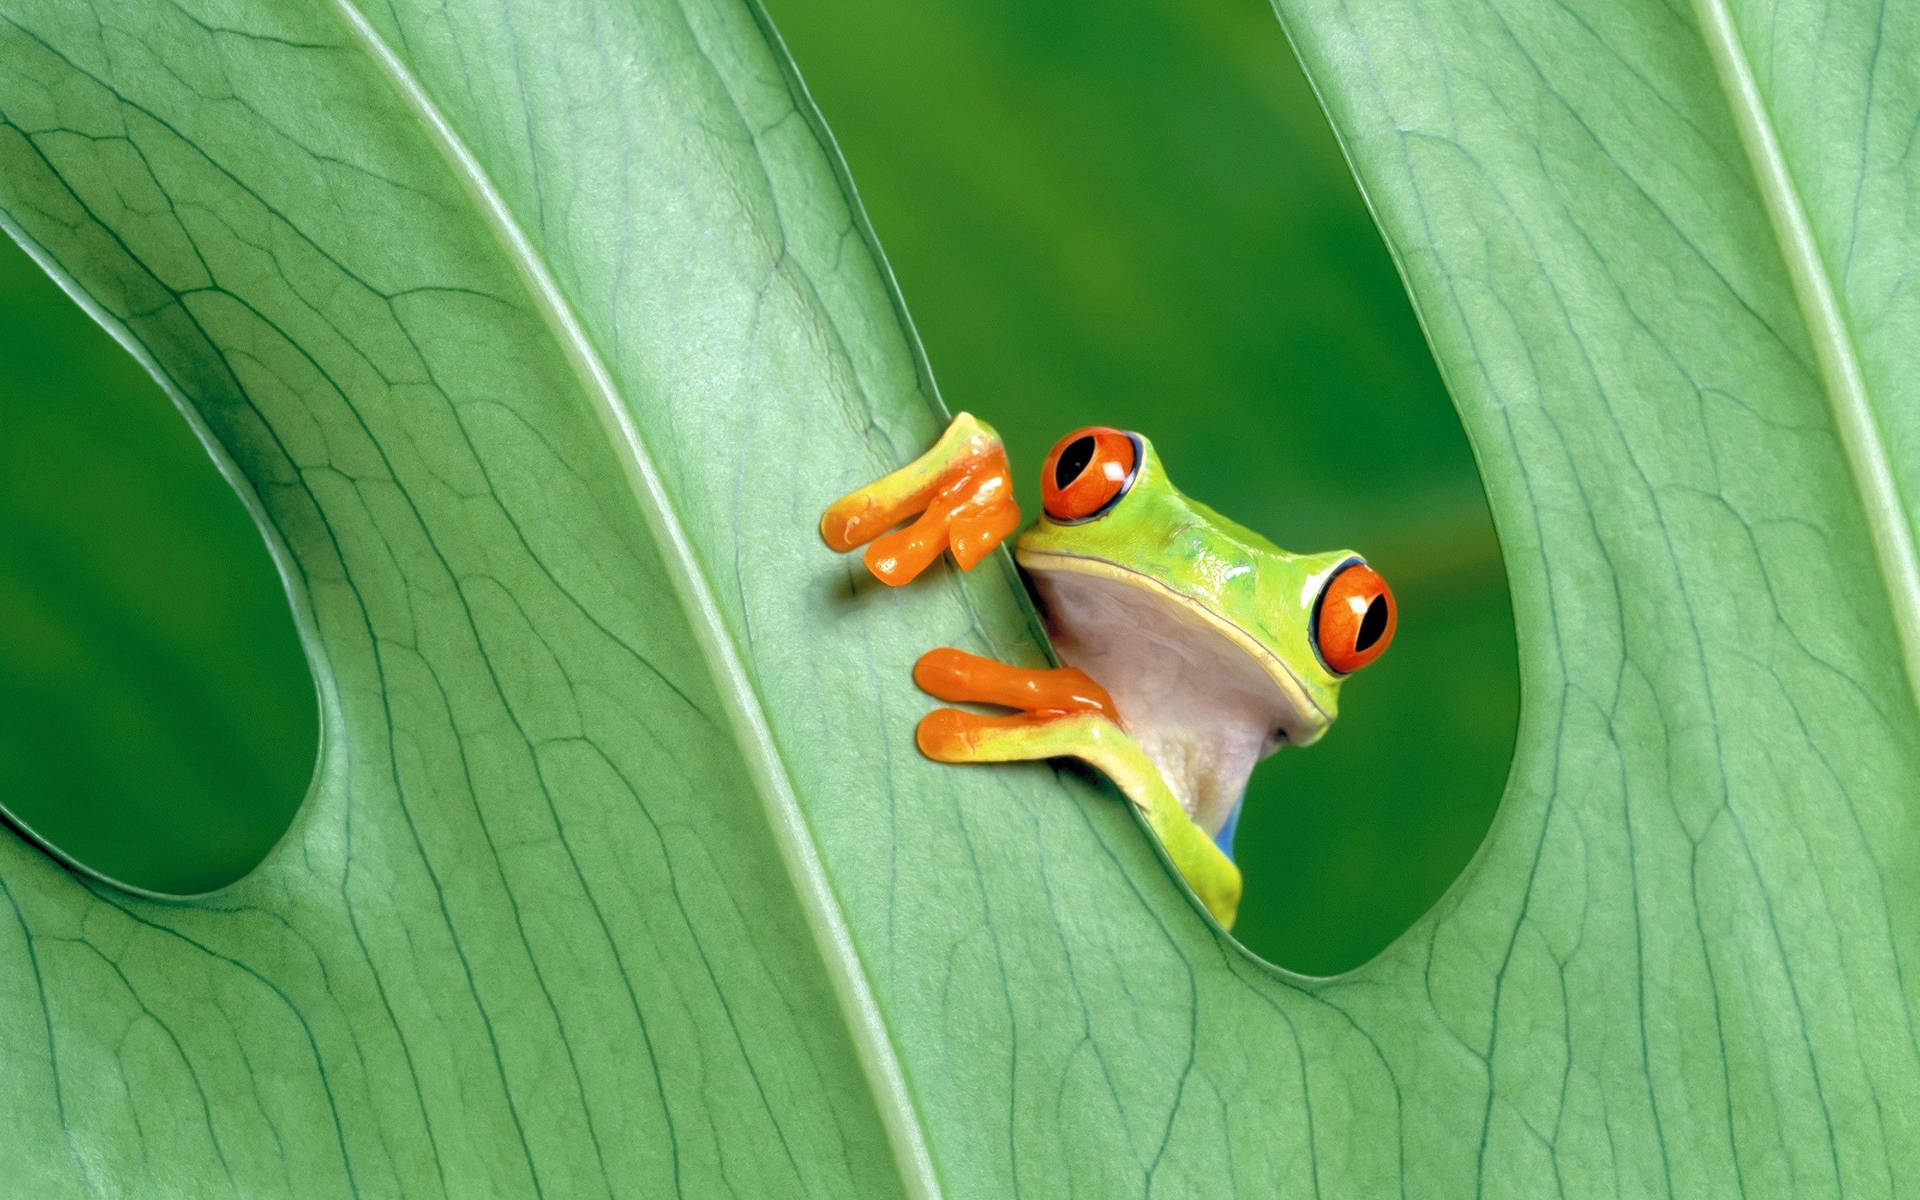
\includegraphics[width=\textwidth]{imagens/sapo1.jpg}
        \caption{Primeira imagem}
    \end{subfigure}
    \hfill
    \begin{subfigure}{0.45\textwidth}
        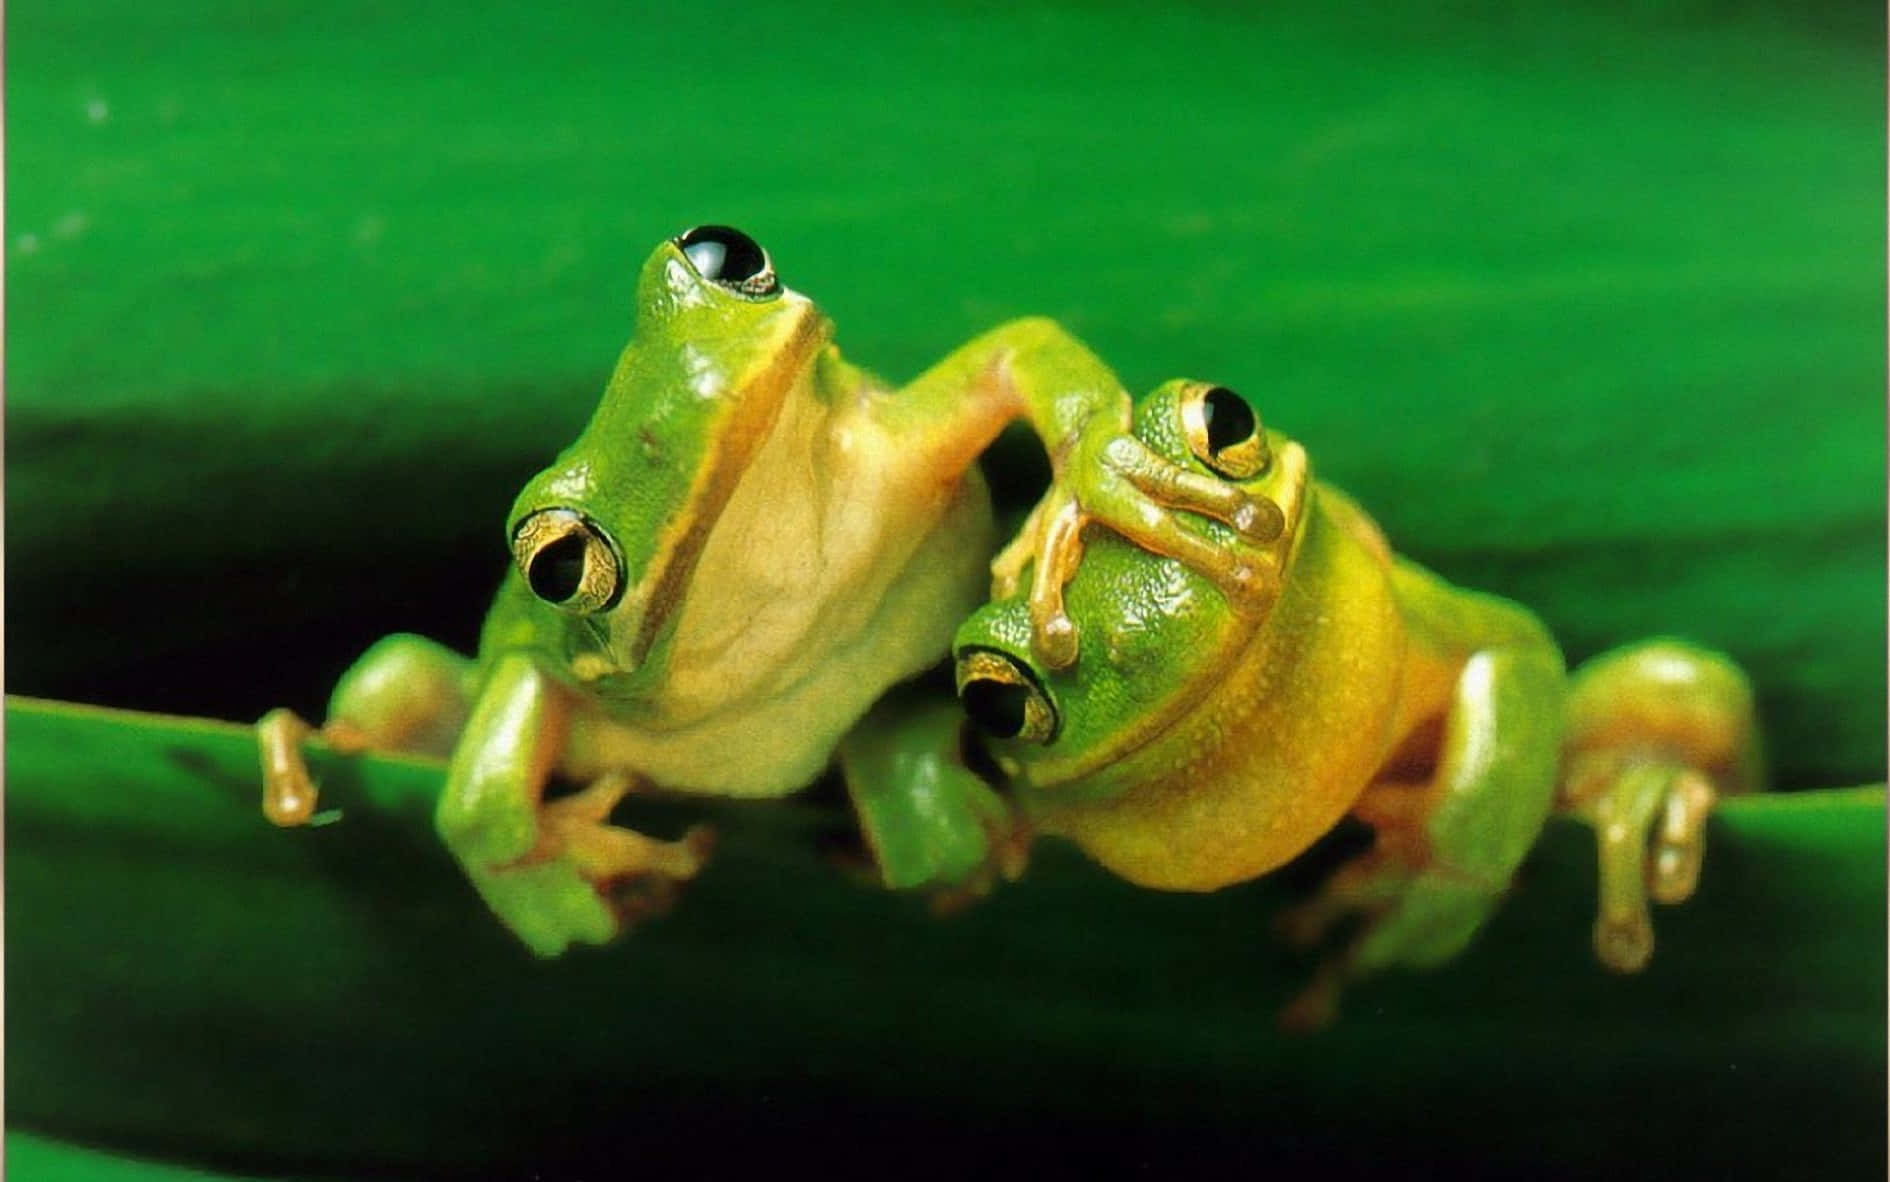
\includegraphics[width=\textwidth]{imagens/sapo2.jpg}
        \caption{Segunda imagem}
    \end{subfigure}
    \caption{Conjunto de imagens}
    \label{fig:duas-imagens}
\end{figure}

\section{Dicas práticas}
\begin{itemize}
    \item Armazene as imagens em uma pasta chamada \verb|imagens| e use:
    \begin{lstlisting}[language=tex, caption=Exemplo de customização do tamanho e ângulo de imagem]
    \graphicspath{{imagens/}} % Define o caminho padrão
    \includegraphics{logo} % Busca por "logo.png" ou "logo.jpg"
    \end{lstlisting}
    \item Erros comuns:
    \begin{itemize}
        \item Imagem não aparece: Verifique o caminho do arquivo e certifique que o pacote \verb|graphicx| está carregado.
        \item Legenda fora do lugar: Use \verb|\centering| dentro do ambiente \verb|figure|.
        \item Formato não suportado: Converta a imagem para um dos formatos suportados. 
    \end{itemize}
    
\end{itemize}

\chapter{Manipulação de Imagens em LaTeX}

\chapterquote{``Citação.''}{Autor}

% --------

\section{Modos matemáticos}

\begin{itemize}
    \item Inline (dentro do texto): Use \verb|\(...\)| ou \verb|$...$|:
    \begin{lstlisting}[language=tex, caption=Equação inline]
    A equação \(E = mc^2\) foi proposta por Einstein.
    \end{lstlisting}
    Saída: A equação \(E = mc^2\) foi proposta por Einstein.
    \item Display: Use \verb|\[...\]| ou \verb|$$...$$|:
    \begin{lstlisting}[language=tex, caption=Equação display]
    A fórmula da energia é:
    \[E = mc^2\]
    \end{lstlisting}
    Saída: \[E = mc^2\]
\end{itemize}

\section{Símbolos básicos}

\begin{itemize}
    \item Letras gregas: \verb|\alpha|, \verb|\beta|, \verb|\gamma|, \verb|\Gamma|, \verb|\Delta|, \verb|\Omega|
    \(\alpha\), \(\beta\), \(\gamma\), \(\Gamma\), \(\Delta\), \(\Omega\)
    \item Operadores e relações: \verb|\times| (multiplicação), \verb|\pm| (mais/menos), \verb|\leq| (menor ou igual), \verb|\geq| (maior ou igual)
    \(\times\), \(\pm\), \(\leq\), \(\geq\)
    \item Setas e símbolos lógicos: \verb|\leftarrow|, \verb|\Leftarrow|, \verb|\rightarrow|, \verb|\Rightarrow|, \verb|\exists| (existe), \verb|\forall| (para todo)
    \(\leftarrow\), \(\Leftarrow\), \(\rightarrow\), \(\Rightarrow\), \(\exists\), \(\forall\)
\end{itemize}

\section{Frações, expoentes e índices}

\begin{itemize}
    \item Frações:
    \begin{lstlisting}[language=tex, caption=Frações em LaTeX]
    \begin{center}
        \(\frac{a}{b}\)\\
    \end{center}
    \[\dfrac{a}{b}\] (uso em display mode)
    \end{lstlisting}
    \begin{center}
        \(\frac{a}{b}\)\\
    \end{center}
    \[\dfrac{a}{b}\]
\end{itemize}

Use \verb|dfrac{a}{b}| para o modo display - o tamanho fica maior.

\section{Matrizes e vetores}

\begin{itemize}
    \item Matrizes simples:
    \begin{lstlisting}[language=tex, caption=Matriz simples]
    \[
    \begin{matrix}
    1 & 2 \\
    3 & 4
    \end{matrix}
    \]
    \end{lstlisting}
    \[
    \begin{matrix}
    1 & 2 \\
    3 & 4
    \end{matrix}
    \]

    \item Matrizes com parênteses (usando \verb|pmatrix|):
    \begin{lstlisting}[language=tex, caption=Matriz com parênteses]
    \[
    \begin{pmatrix}
    a & b \\
    c & d
    \end{pmatrix}
    \]
    \end{lstlisting}
    \[
    \begin{pmatrix}
    a & b \\
    c & d
    \end{pmatrix}
    \]    

    \item Matrizes com colchetes (usando \verb|bmatrix|):
    \begin{lstlisting}[language=tex, caption=Matriz com colchetes]
    \[
    \begin{bmatrix}
    X & Y \\
    Z & W
    \end{bmatrix}
    \]
    \end{lstlisting}
    \[
    \begin{bmatrix}
    X & Y \\
    Z & W
    \end{bmatrix}
    \] 
\end{itemize}

\section{Ambientes avançados}

\begin{itemize}
    \item Equações numeradas:
    \begin{lstlisting}[language=tex, caption=Equação numerada]
    \begin{equation}
        \label{eq:energia}
        E = mc^{2}
    \end{equation}
    \end{lstlisting}
    \begin{equation}
        \label{eq:energia}
        E = mc^{2}
    \end{equation}

    \item Alinhamento de equações (ambiente \verb|align|):
    \begin{lstlisting}[language=tex, caption=Equações alinhadas]
    \begin{align}
        x & + y = 5 \\
        2x - y = 3 &
    \end{align}
    \end{lstlisting}
    \begin{align}
        x & + y = 5 \\
        2x - y = 3 &
    \end{align}
\end{itemize}

Para não enumerar as equações, use o ambiente \verb|align*|:

\begin{lstlisting}[language=tex, caption=Equações alinhadas e não enumeradas]
\begin{align*}
    x & + y = 5 \\
    2x - y = 3 &
\end{align*}
\end{lstlisting}
\begin{align*}
    x & + y = 5 \\
    2x - y = 3 &
\end{align*}

\section{Sistemas de equações}

Use o ambiente \verb|cases| (requer o pacote \verb|amsmath|):

\begin{lstlisting}[language=tex, caption=Sistema de equações]
    \[
    f(x) = 
    \begin{cases}
    x^{2} & \text{se } x \geq 0 \\
    -x & \text{se } x < 0
    \end{cases}
    \]
\end{lstlisting}

\[
f(x) = 
\begin{cases}
x^{2} & \text{se } x \geq 0 \\
-x & \text{se } x < 0
\end{cases}
\]

\section{Dicas práticas}

\begin{itemize}
    \item Pacote essencial:
    \begin{lstlisting}[language=tex, caption=Carregue o pacote \texttt{amsmath}]
    \usepackage{amsmath} % Carregue sempre!
    \end{lstlisting}
    \item Erros comuns:
    \begin{itemize}
        \item Esquecer de usar \verb|\| antes de símbolos especiais (ex: \verb|\alpha|, não \verb|alpha|).
        \item Não fechar chaves em expoentes/subscritos (ex: \verb|x^{2}| em vez de \verb|x^2|).
    \end{itemize}
\end{itemize}

Dica: Use o \href{https://detexify.kirelabs.org/classify.html}{Detexify} para encontrar símbolos matemáticos desconhecidos!
\chapter{Bibliografia e citações em LaTeX}

\chapterquote{``Citação.''}{Autor}

% --------

\section{Introdução ao gerenciamento de referências}

O LaTeX oferece ferramentas poderosas para criar e gerenciar referências bibliográficas de forma automatizada, garantindo consistência e padronização em documentos acadêmicos.

\section{Citações básicas}

Use o comando \verb|\cite{citação}| para citar uma referência.

\begin{lstlisting}[language=tex, caption=Exemplo simples de citação]
    Segundo \cite{einstein}, a teoria da relatividade...
\end{lstlisting}

\section{Criando uma bibliografia manual}

Para documentos pequenos, use o ambiente \verb|thebibliography|:

\begin{lstlisting}[language=tex, caption=Equação inline]
    \begin{thebibliography}{9} % O número 9 indica a largura máxima de rótulos
        \bibitem{einstein}  
            Einstein, A. (1905).  
            \textit{Zur Elektrodynamik bewegter Körper}.  
            Annalen der Physik, 17(10), 891–921.  
    \end{thebibliography}
\end{lstlisting}

\section{Usando o BibTeX (Recomendado)}

O \textbf{BibTeX} automatiza a criação de bibliografias. Siga os passos:

\begin{enumerate}
    \item Crie um arquivo \verb|.bib| (ex: \verb|referencias.bib|) com entradas no formato:
    \begin{lstlisting}[language=tex, caption=Exemplo de formatação em um arquivo \texttt{.bib}]
    @article{einstein1905,
        author  = "Albert Einstein",
        title   = "Zur Elektrodynamik bewegter Körper",
        journal = "Annalen der Physik",
        year    = "1905",
        volume  = "322",
        pages   = "891--921"
    }
    \end{lstlisting}

    \item Inclua o arquivo no documento:
    \begin{lstlisting}[language=tex, caption=Incluindo o arquivo de bibliografias no documento]
    \bibliographystyle{plain} % Estilo (ex: abnt, ieee, apa)
    \bibliography{referencias} % Nome do arquivo .bib (sem extensão)
    \end{lstlisting}
\end{enumerate}

\section{Estilos de citação}

Altere o estilo com \verb|\bibliographystyle|:

\begin{itemize}
    \item \verb|plain|: Numérico (padrão).
    \item \verb|abnt|: Normas ABNT (requer o pacote \verb|abntex2|).
    \item \verb|apa|: Formato APA.
    \item \verb|ieee|: Padrão IEEE.
\end{itemize}

\begin{lstlisting}[language=tex, caption=Definindo o estilo da bibliografia]
    \bibliographystyle{ieee}  
    \bibliography{referencias}  
\end{lstlisting}

\section{Dicas práticas}
\begin{itemize}
    \item \textbf{Zotero + Better BibTeX}: Exporte referências diretamente para \verb|.bib|.
    \item \textbf{JabRef}: Editor gratuito para gerenciar arquivos \verb|.bib|.
    \item \textbf{DOI para BibTeX}: Sites como \href{https://www.doi2bib.org/}{doi2bib} convertem DOIs em entradas BibTeX.
    \item Erros comuns:
    \begin{itemize}
        \item Referência não aparece: Verifique se a chave em \verb|\cite{citação}| corresponde à entrada no arquivo \verb|.bib|.
        \item Estilo incorreto: Confira se o estilo desejado e adequado está instalado.
    \end{itemize}
\end{itemize}

\chapter{Layouts profissionais}

\chapterquote{``Citação.''}{Autor}

% --------

\section{Controle de geometria da página}

Use o pacote \verb|geometry| para ajustar margens, cabeçalhos e rodapés:

\begin{lstlisting}[language=tex, caption=Configuração da geometria das páginas]
    \usepackage[top=3cm, bottom=2.5cm, left=3cm, right=2cm, headheight=15pt]{geometry}
\end{lstlisting}    

Parâmetros úteis:
\begin{itemize}
    \item \verb|includeheadfoot|: Inclui cabeçalho/rodapé no cálculo das margens.
    \item \verb|landscape|: Modo paisagem (\verb|\usepackage{pdflscape}| para páginas específicas).
\end{itemize}

\section{Cabeçalhos e rodapés personalizados}

Use o pacote \verb|fancyhdr| para designs avançados:

\begin{lstlisting}[language=tex, caption=Usando o pacote \texttt{fancyhdr} para personalização de estilo]
    \usepackage{fancyhdr}
    \pagestyle{fancy}
    \fancyhf{} % Limpa estilos padrão
    \rhead{\textit{Nome do Documento}} 
    \lfoot{\thepage}
    \rfoot{\today}
    \renewcommand{\headrulewidth}{1pt} % Linha no cabeçalho
\end{lstlisting}   

Estilos diferentes para páginas específicas:

\begin{lstlisting}[language=tex, caption=Estilizando páginas específicas]
    \fancypagestyle{plain}{ % Estilo para páginas de capítulo
        \fancyhf{}
        \rfoot{Página \thepage}
    }
\end{lstlisting}   

\section{Personalização de títulos e seções}

\begin{lstlisting}[language=tex, caption=Pacote \texttt{titlesec} para alterar títulos e seções]
    \usepackage{titlesec}
    \titleformat{\section}[block] % Formato do título
        {\bfseries\Large\color{blue}} % Fonte
        {\thesection} % Rótulo
        {1em} % Espaço entre rótulo e título
        {} 
    
    \titlespacing{\section}{0pt}{12pt}{6pt} % Espaçamento: esquerda, acima, abaixo
\end{lstlisting}  

\section{Fontes e tipografia}

\begin{itemize}
    \item Pacotes de fontes:
    \begin{lstlisting}[language=tex, caption=Pacotes de fontes mais usados]
    \usepackage{lmodern}       % Latin Modern (padrão aprimorado)
    \usepackage{kpfonts}       % Fonte Kepler (estilo clássico)
    \usepackage{roboto}        % Fonte moderna (requer XeLaTeX/LuaLaTeX)
    \end{lstlisting} 
    
    \item Configuração global:
    \begin{lstlisting}[language=tex, caption=Fonte padrão para o documento]
    \renewcommand{\familydefault}{\sfdefault} % Muda fonte padrão para sans-serif
    \end{lstlisting}      
\end{itemize}

\section{Cores temáticas}

Use o pacote \verb|xcolor| para definir esquemas de cores:

\begin{lstlisting}[language=tex, caption=Alterando a cores de títulos e seções]
    \definecolor{corprimaria}{RGB}{0, 102, 204} % Azul institucional
    \definecolor{cortitulo}{HTML}{800080}       % Roxo em hexadecimal
    
    % Aplicação em títulos:
    \titleformat{\chapter}{\color{cortitulo}\Huge\bfseries}{\thechapter}{1em}{}
\end{lstlisting}

\section{Caixas e destaques}

Crie caixas estilizadas com \verb|mdframed| ou \verb|tcolorbox|:

\begin{lstlisting}[language=tex, caption=Exemplo de caixa de destaque]
    \usepackage{tcolorbox}
    \newtcolorbox{caixadestaque}{
        colback=blue!10!white, % Cor de fundo
        colframe=blue!50!black, % Cor da borda
        arc=4pt, % Arredondamento
        boxrule=1.5pt % Espessura da borda
    }
    
    % Uso:
    \begin{caixadestaque}
        Texto destacado aqui.
    \end{caixadestaque}
\end{lstlisting}

\newtcolorbox{caixadestaque}{
    colback=blue!10!white, % Cor de fundo
    colframe=blue!50!black, % Cor da borda
    arc=4pt, % Arredondamento
    boxrule=1.5pt % Espessura da borda
}

% Uso:
\begin{caixadestaque}
    Texto destacado aqui.
\end{caixadestaque}

\section{Ambientes personalizados}

Crie ambientes para teoremas, exemplos ou definições:

\begin{lstlisting}[language=tex, caption=Caixa de destaque simples para teorema]
    \usepackage{amsthm}
    \newtheorem{teorema}{Teorema}[section] % Numeração por seção
    
    % Uso:
    \begin{teorema}[Pitágoras]
        Em um triângulo retângulo, \(a^2 + b^2 = c^2\).
    \end{teorema}
\end{lstlisting}

\newtheorem{teorema1}{Teorema}[section] % Numeração por seção

% Uso:
\begin{teorema1}[Pitágoras]
    Em um triângulo retângulo, \(a^2 + b^2 = c^2\).
\end{teorema1}

Você pode se aprofundar bastante aqui. Veja os exemplos abaixo:

\begin{tcolorbox}[enhanced,
colback=red!10!white,colframe=red!75!black,
colbacktitle=red!50!yellow,fonttitle=\bfseries,
frame hidden,
title=My title,
boxrule=0pt,titlerule=1mm,
titlerule style=red!50!black ]
This is a \textbf{tcolorbox}.
\end{tcolorbox}

\begin{tcolorbox}[tile,flip title={sharp corners},
title=My title,colback=red!10,
colbacktitle=red!75!black]
This is a \textbf{tcolorbox}.
\end{tcolorbox}

\begin{tcolorbox}[enhanced,title=My title,
attach boxed title to bottom*]
This is a \textbf{tcolorbox}.
\end{tcolorbox} 

\begin{tcolorbox}[enhanced,title=My title,
attach boxed title to top center={yshift*=-3mm},
boxed title style={size=small,colback=blue}]
This is a \textbf{tcolorbox}.
\end{tcolorbox}

\begin{tcolorbox}[enhanced,title=My title,
colframe=red!50!black,colback=red!10!white,
arc=1mm,colbacktitle=red!10!white,
fonttitle=\bfseries,coltitle=red!50!black,
attach boxed title to top text left=
{yshift=-0.50mm},
boxed title style={skin=enhancedfirst jigsaw,
size=small,arc=1mm,bottom=-1mm,
interior style={fill=none,
top color=red!30!white,
bottom color=red!20!white}}]
This is a \textbf{tcolorbox}.
\end{tcolorbox}

% \usepackage{varwidth}
\newtcolorbox{mybox1}[2][]{enhanced,skin=enhancedlast jigsaw,
attach boxed title to top left={xshift=-4mm,yshift=-0.5mm},
fonttitle=\bfseries\sffamily,varwidth boxed title=0.7\linewidth,
colbacktitle=blue!45!white,colframe=red!50!black,
interior style={top color=blue!10!white,bottom color=red!10!white},
boxed title style={empty,arc=0pt,outer arc=0pt,boxrule=0pt},
underlay boxed title={
\fill[blue!45!white] (title.north west) -- (title.north east)
-- +(\tcboxedtitleheight-1mm,-\tcboxedtitleheight+1mm)
-- ([xshift=4mm,yshift=0.5mm]frame.north east) -- +(0mm,-1mm)
-- (title.south west) -- cycle;
\fill[blue!45!white!50!black] ([yshift=-0.5mm]frame.north west)
-- +(-0.4,0) -- +(0,-0.3) -- cycle;
\fill[blue!45!white!50!black] ([yshift=-0.5mm]frame.north east)
-- +(0,-0.3) -- +(0.4,0) -- cycle; },
title={#2},#1}
\begin{mybox1}{My title}
\lipsum[2]
\end{mybox1}

\newtcolorbox{mybox2}[1]{hbox boxed title,
enhanced,attach boxed title to top center=
{yshift=-3mm,yshifttext=-1mm},
boxed title style={size=small,colback=red},
title={#1}}
\begin{mybox2}{Short title}
This is a \textbf{tcolorbox}.
\end{mybox2}\bigskip
\begin{mybox2}{This title is not really very short}
This is a \textbf{tcolorbox}.
\end{mybox2}

\begin{tcolorbox}[drop shadow southeast,
enhanced,colback=red!5!white,colframe=red!75!black]
This is a tcolorbox.
\end{tcolorbox}

\newtcolorbox{mybox3}[1][]{enhanced,
fuzzy shadow={1.0mm}{-1.0mm}{0.12mm}{0mm}{blue!50!white},
fuzzy shadow={-1.0mm}{-1.0mm}{0.12mm}{0mm}{red!50!white},
fuzzy shadow={-1.0mm}{1.0mm}{0.12mm}{0mm}{green!50!white},
fuzzy shadow={1.0mm}{1.0mm}{0.12mm}{0mm}{yellow!50!white},#1
}
\begin{mybox3}[title=A multi shadow box]
This is a tcolorbox.
\end{mybox3}

Esses são apenas alguns exemplos retirados da \href{https://www.tug.org/docs/latex/tcolorbox/tcolorbox.pdf}{documentação do pacote \texttt{tcolorbox}}. Existem muitos outros modelos feitos pela comunidade, além de várias outras aplicações e usos desse pacote.

\section{Dicas práticas}

\begin{itemize}
    \item Consistência: Defina um arquivo \verb|.sty| com todas as personalizações para reutilização.
    \item Templates: Use \href{https://www.overleaf.com/latex/templates}{modelos do Overleaf} como base.
    \item Evite excessos: Priorize clareza e normas da instituição.
\end{itemize}
\chapter{Gráficos e diagramas}

\chapterquote{``Citação.''}{Autor}

% --------

\section{Introdução ao \texttt{TikZ} e \texttt{pgfplots}}

Use o pacote \verb|geometry| para ajustar margens, cabeçalhos e rodapés:

\begin{itemize}
    \item \verb|TikZ|: Pacote para criação de gráficos vetoriais, diagramas e ilustrações complexas diretamente no LaTeX.
    \item \verb|pgfplots|: Extensão do TikZ para plotagem de dados e funções matemáticas.
\end{itemize}   

\begin{lstlisting}[language=tex, caption=Carregue os pacotes essenciais]
    \usepackage{tikz}
    \usepackage{pgfplots}
    \pgfplotsset{compat=1.18} % Define a versão para compatibilidade
    \usetikzlibrary{shapes, arrows.meta, positioning} % Bibliotecas úteis
\end{lstlisting} 

\section{Exemplos}

\subsection{Linhas e pontos}

\begin{lstlisting}[language=tex, caption={Linhas e pontos}]
    \begin{center}
        \begin{tikzpicture}
            \draw[thick] (0,0) -- (2,0) -- (1,1.5) -- cycle;
            \foreach \point in {(0,0), (2,0), (1,1.5)}
            \fill \point circle (2pt);
        \end{tikzpicture}
    \end{center}
\end{lstlisting} 


\begin{center}
    \begin{tikzpicture}
        \draw[thick] (0,0) -- (2,0) -- (1,1.5) -- cycle;
        \foreach \point in {(0,0), (2,0), (1,1.5)}
        \fill \point circle (2pt);
    \end{tikzpicture}
\end{center}

\begin{itemize}
    \item Espessuras: \verb|ultra thin|, \verb|very thin|, \verb|thin|, \verb|semithick|, \verb|thick|, \verb|very thick|, \verb|ultra thick|
    \item Espessura específica:\\\verb|\draw[line width=1.5pt] (0,0) -- (2,0) -- (1,1.5) -- cycle;|
\end{itemize}

\subsection{Retângulo e círculo}

\begin{lstlisting}[language=tex, caption=Retângulo e círculo]
    \begin{center}
        \begin{tikzpicture}
            \draw[thick, dashed, red] (-1,0) rectangle (1,2);
            \draw[thick, fill=blue!20] (3,0) circle (1cm);
        \end{tikzpicture}
    \end{center}
\end{lstlisting} 

\begin{center}
    \begin{tikzpicture}
        \draw[thick, dashed, red] (-1,0) rectangle (1,2);
        \draw[thick, fill=blue!20] (3,0) circle (1cm);
    \end{tikzpicture}
\end{center}

\subsection{Diagramas de fluxo}

\begin{lstlisting}[language=tex, caption=Diagramas de fluxo]
    \begin{center}
        \begin{tikzpicture}
            \node (start) at (-2,0) [draw, rectangle] {Início};
            \node (step1) at (0,0) [draw, circle] {Passo 1};
            \node (end) at (2,0) [draw, rectangle] {Fim};
        
            \draw[->] (start) -- (step1);
            \draw[->] (step1) -- (end);
        \end{tikzpicture}
    \end{center}
\end{lstlisting} 

\begin{center}
    \begin{tikzpicture}
        \node (start) at (-2,0) [draw, rectangle] {Início};
        \node (step1) at (0,0) [draw, circle] {Passo 1};
        \node (end) at (2,0) [draw, rectangle] {Fim};
    
        \draw[->] (start) -- (step1);
        \draw[->] (step1) -- (end);
    \end{tikzpicture}
\end{center}

\subsection{Gráfico de Função Senoidal}

\begin{lstlisting}[language=tex, caption=Gráfico de Função Senoidal]
    \begin{center}
        \begin{tikzpicture}
            \begin{axis}[
                axis lines = middle,
                xlabel = \(x\),
                ylabel = {\(f(x) = \sin(x)\)},
                xmin = -6, xmax = 6,
                ymin = -1.5, ymax = 1.5,
                grid = major,
                width=10cm,
                height=6cm
            ]
            \addplot[domain=-2*pi:2*pi, samples=100, color=green] {sin(deg(x))};
            \end{axis}
        \end{tikzpicture}
    \end{center}
\end{lstlisting} 

\begin{center}
    \begin{tikzpicture}
        \begin{axis}[
            axis lines = middle,
            xlabel = \(x\),
            ylabel = {\(f(x) = \sin(x)\)},
            xmin = -6, xmax = 6,
            ymin = -1.5, ymax = 1.5,
            grid = major,
            width=10cm,
            height=6cm
        ]
        \addplot[domain=-2*pi:2*pi, samples=100, color=green] {sin(deg(x))};
        \end{axis}
    \end{tikzpicture}
\end{center}

\subsection{Gráfico de barras e dados}

\begin{lstlisting}[language=tex, caption=Gráfico de barras]
    \begin{center}
        \begin{tikzpicture}
            \begin{axis}[
                ybar,
                symbolic x coords={A,B,C,D},
                xtick=data,
                nodes near coords,
                xlabel=Categorias,
                ylabel=Valores,
                title={Exemplo de Gráfico de Barras},
                legend pos=north west
            ]
            \addplot coordinates {(A,20) (B,45) (C,30) (D,55)};
            \addplot coordinates {(A,25) (B,40) (C,35) (D,45)};
            \legend{2023, 2024}
            \end{axis}
        \end{tikzpicture}
    \end{center}
\end{lstlisting} 

\begin{center}
    \begin{tikzpicture}
        \begin{axis}[
            ybar,
            symbolic x coords={A,B,C,D},
            xtick=data,
            nodes near coords,
            xlabel=Categorias,
            ylabel=Valores,
            title={Exemplo de Gráfico de Barras},
            legend pos=north west
        ]
        \addplot coordinates {(A,20) (B,45) (C,30) (D,55)};
        \addplot coordinates {(A,25) (B,40) (C,35) (D,45)};
        \legend{2023, 2024}
        \end{axis}
    \end{tikzpicture}
\end{center}

\subsection{Diagrama de Venn}

\begin{lstlisting}[language=tex, caption=Diagrama de Venn]
    \begin{center}
        \begin{tikzpicture}
            \centering
            \begin{scope}[shift={(3cm,-5cm)}, fill opacity=0.5]
                \fill[red] \firstcircle;
                \fill[green] \secondcircle;
                \fill[blue] \thirdcircle;
                \draw \firstcircle node[below] {$A$};
                \draw \secondcircle node [above] {$B$};
                \draw \thirdcircle node [below] {$C$};
            \end{scope}
        \end{tikzpicture}
    \end{center}
\end{lstlisting} 

\def\firstcircle{(0,0) circle (1.5cm)}
\def\secondcircle{(60:2cm) circle (1.5cm)}
\def\thirdcircle{(0:2cm) circle (1.5cm)}

\begin{center}
    \begin{tikzpicture}
        \centering
        \begin{scope}[shift={(3cm,-5cm)}, fill opacity=0.5]
            \fill[red] \firstcircle;
            \fill[green] \secondcircle;
            \fill[blue] \thirdcircle;
            \draw \firstcircle node[below] {$A$};
            \draw \secondcircle node [above] {$B$};
            \draw \thirdcircle node [below] {$C$};
        \end{scope}
    \end{tikzpicture}
\end{center}

\subsection{Superfície 3D (função matemática)}

\begin{lstlisting}[language=tex, caption=Superfície 3D de função matemática]
    \begin{center}
        \begin{tikzpicture}
            \begin{axis}[
                view={60}{30}, % Ângulo de visualização (azimute, elevação)
                xlabel = \(x\),
                ylabel = \(y\),
                zlabel = \(z\),
                title = {Superfície \(z = \sin(x) \cdot \sin(y)\)},
                colormap/viridis, % Esquema de cores
            ]
            \addplot3[
                surf,
                domain = -3:3,
                domain y = -3:3,
                samples = 25,
            ] 
                {sin(deg(x)) * sin(deg(y))};
            \end{axis}
        \end{tikzpicture}
    \end{center}
\end{lstlisting} 

\begin{center}
    \begin{tikzpicture}
        \begin{axis}[
            view={60}{30}, % Ângulo de visualização (azimute, elevação)
            xlabel = \(x\),
            ylabel = \(y\),
            zlabel = \(z\),
            title = {Superfície \(z = \sin(x) \cdot \sin(y)\)},
            colormap/viridis, % Esquema de cores
        ]
        \addplot3[
            surf,
            domain = -3:3,
            domain y = -3:3,
            samples = 25,
        ] 
            {sin(deg(x)) * sin(deg(y))};
        \end{axis}
    \end{tikzpicture}
\end{center}

\subsection{Gráfico de Dispersão 3D}

\begin{lstlisting}[language=tex, caption=Gráfico de Dispersão 3D]
    \begin{center}
        \begin{tikzpicture}
            \begin{axis}[
                view={120}{40},
                xlabel = \(X\),
                ylabel = \(Y\),
                zlabel = \(Z\),
                title = {Dispersão 3D},
                grid = major,
            ]
            \addplot3[
                only marks,
                mark = *,
                mark size = 1.5pt,
                color = red,
            ] coordinates {
                (1,2,3) (2,3,4) (3,4,5)
                (4,5,6) (5,6,7) (6,7,8)
            };
            \end{axis}
        \end{tikzpicture}
    \end{center}
\end{lstlisting} 

\begin{center}
    \begin{tikzpicture}
        \begin{axis}[
            view={120}{40},
            xlabel = \(X\),
            ylabel = \(Y\),
            zlabel = \(Z\),
            title = {Dispersão 3D},
            grid = major,
        ]
        \addplot3[
            only marks,
            mark = *,
            mark size = 1.5pt,
            color = red,
        ] coordinates {
            (1,2,3) (2,3,4) (3,4,5)
            (4,5,6) (5,6,7) (6,7,8)
        };
        \end{axis}
    \end{tikzpicture}
\end{center}

\subsection{Gráfico Paramétrico (hélice)}

\begin{lstlisting}[language=tex, caption=Gráfico Paramétrico (hélice)]
    \begin{center}
        \begin{tikzpicture}
            \begin{axis}[
                view={60}{30}, % Alterado para uma visão mais tridimensional
                xlabel = {\textit{x(t)}},
                ylabel = {\textit{y(t)}},
                zlabel = {\textit{z(t)}},
                title = {\textbf{Hélice Paramétrica}},
                grid = major, % Adiciona grade para melhor visualização
                xtick = {-1, 0, 1},
                ytick = {-1, 0, 1},
                ztick = {0, 2, 4, 6}, % Ajustando os ticks do eixo z
                enlargelimits = 0.1,
                legend pos=north east, % Posição da legenda
            ]
            \addplot3[
                domain = 0:4*pi,
                samples = 100,
                samples y = 0,
                color = blue,
                very thick, % Linha mais grossa para destaque
            ] 
                ({cos(deg(x))}, {sin(deg(x))}, {x/2}) 
                node[pos=0.9,anchor=south west] {\small Hélice};
            \end{axis}
        \end{tikzpicture}
\end{center}
\end{lstlisting} 

\begin{center}
    \begin{tikzpicture}
        \begin{axis}[
            view={60}{30}, % Alterado para uma visão mais tridimensional
            xlabel = {\textit{x(t)}},
            ylabel = {\textit{y(t)}},
            zlabel = {\textit{z(t)}},
            title = {\textbf{Hélice Paramétrica}},
            grid = major, % Adiciona grade para melhor visualização
            xtick = {-1, 0, 1},
            ytick = {-1, 0, 1},
            ztick = {0, 2, 4, 6}, % Ajustando os ticks do eixo z
            enlargelimits = 0.1,
            legend pos=north east, % Posição da legenda
        ]
        \addplot3[
            domain = 0:4*pi,
            samples = 100,
            samples y = 0,
            color = blue,
            very thick, % Linha mais grossa para destaque
        ] 
            ({cos(deg(x))}, {sin(deg(x))}, {x/2}) 
            node[pos=0.9,anchor=south west] {\small Hélice};
        \end{axis}
    \end{tikzpicture}
\end{center}

\subsection{Gráfico de contorno 3D}

\begin{lstlisting}[language=tex, caption=Gráfico de contorno 3D]
    \begin{center}
        \begin{tikzpicture}
            \begin{axis}[
                view={45}{30}, % Ângulo ajustado para melhor visualização
                colormap={customgreen}{ % Paleta verde suave e equilibrada
                    rgb255(0cm)=(0,100,0)   % Verde escuro
                    rgb255(1cm)=(34,139,34) % Verde floresta
                    rgb255(2cm)=(50,205,50) % Verde lima
                    rgb255(3cm)=(144,238,144) % Verde claro
                    rgb255(4cm)=(230,255,230) % Verde quase branco
                },
                enlargelimits=false,
                hide axis, % Remove eixos para um visual mais clean
                colorbar, % Adiciona barra lateral de cores
                colorbar style={
                    ylabel={Temperatura (°C)}, % Rótulo da escala
                    ytick={-1,0,1,2,3,4}, % Marcas da barra de cores
                }
            ]
                % Superfície 3D ondulada com interpolação de cores
                \addplot3[
                    surf, % Superfície 3D
                    shader=interp, % Suaviza a transição de cores
                    domain=-2:2, y domain=-2:2, % Domínio dos eixos
                    samples=40, % Número de pontos para maior suavidade
                    samples y=40
                ]
                {sin(deg(x)) * cos(deg(y))}; % Função matemática ondulada
    
                % Adicionando a grid na superfície para um efeito visual aprimorado
                \addplot3[
                    mesh, % Plota uma malha (grid) na superfície
                    domain=-2:2, y domain=-2:2, 
                    samples=20, % Define quantos segmentos terá a malha
                    samples y=20,
                    thick, % Deixa as linhas da grid mais visíveis
                    black!30 % Define a cor da grid como cinza escuro (30% preto)
                ]
                {sin(deg(x)) * cos(deg(y))};
            \end{axis}
        \end{tikzpicture}
    \end{center}
\end{lstlisting} 

\begin{center}
    \begin{tikzpicture}
        \begin{axis}[
            view={45}{30}, % Ângulo ajustado para melhor visualização
            colormap={customgreen}{ % Paleta verde suave e equilibrada
                rgb255(0cm)=(0,100,0)   % Verde escuro
                rgb255(1cm)=(34,139,34) % Verde floresta
                rgb255(2cm)=(50,205,50) % Verde lima
                rgb255(3cm)=(144,238,144) % Verde claro
                rgb255(4cm)=(230,255,230) % Verde quase branco
            },
            enlargelimits=false,
            hide axis, % Remove eixos para um visual mais clean
            colorbar, % Adiciona barra lateral de cores
            colorbar style={
                ylabel={Temperatura (°C)}, % Rótulo da escala
                ytick={-1,0,1,2,3,4}, % Marcas da barra de cores
            }
        ]
            % Superfície 3D ondulada com interpolação de cores
            \addplot3[
                surf, % Superfície 3D
                shader=interp, % Suaviza a transição de cores
                domain=-2:2, y domain=-2:2, % Domínio dos eixos
                samples=40, % Número de pontos para maior suavidade
                samples y=40
            ]
            {sin(deg(x)) * cos(deg(y))}; % Função matemática ondulada

            % Adicionando a grid na superfície para um efeito visual aprimorado
            \addplot3[
                mesh, % Plota uma malha (grid) na superfície
                domain=-2:2, y domain=-2:2, 
                samples=20, % Define quantos segmentos terá a malha
                samples y=20,
                thick, % Deixa as linhas da grid mais visíveis
                black!30 % Define a cor da grid como cinza escuro (30% preto)
            ]
            {sin(deg(x)) * cos(deg(y))};
        \end{axis}
    \end{tikzpicture}
\end{center}

\section{Dicas práticas}

\begin{itemize}
    \item \href{https://tikz.dev/}{Manual do \texttt{TikZ}}.
    \item \href{https://pgfplots.sourceforge.net/}{Manual do \texttt{pgfplots}}.
    \item Templates: Explore modelos prontos em \href{https://texample.net/}{TeXample.net}.
\end{itemize}

\end{document}